% ==============================================================================
% BÁO CÁO ĐỒ ÁN MÔN HỌC: THIẾT KẾ LUẬN LÝ SỐ (DIGITAL LOGIC DESIGN)
% Đề tài: Thiết kế CPU MIPS 32-bit Pipeline 5 tầng (IF, ID, EX, MEM, WB)
%         hiện thực trên phần mềm Intel/Altera Quartus II (BDF & Verilog HDL)
% Biên dịch chuẩn trên Overleaf bằng trình biên dịch: pdfLaTeX
% ==============================================================================
\documentclass[12pt,a4paper]{report}

% --- 1. GÓI NGÔN NGỮ TIẾNG VIỆT & FONT CHỮ CHUẨN ---
\usepackage[utf8]{inputenc}
\usepackage[T5]{fontenc}
\usepackage[vietnamese]{babel}
\usepackage{mathptmx} % Font Times New Roman chuẩn báo cáo kỹ thuật

% --- 2. CẤU HÌNH LỀ TRANG & GIÃN DÒNG ---
\usepackage[left=3.0cm,right=2.0cm,top=2.5cm,bottom=2.5cm]{geometry}
\usepackage{setspace}
\onehalfspacing
\setlength{\parindent}{1.0cm}
\setlength{\parskip}{6pt}

% --- 3. GÓI TOÁN HỌC, BẢNG BIỂU & HÌNH ẢNH ---
\usepackage{amsmath,amssymb,amsfonts}
\usepackage{graphicx}
\usepackage{float}
\usepackage{subcaption}
\usepackage{booktabs}
\usepackage{multirow}
\usepackage{longtable}
\usepackage{array}
\usepackage[table,xcdraw]{xcolor}
\usepackage{tikz}
\usetikzlibrary{calc}
\definecolor{uitborder}{HTML}{215E99}

% --- 4. GÓI HEADER/FOOTER & ĐỊNH DẠNG CHƯƠNG MỤC ---
\usepackage{fancyhdr}
\pagestyle{fancy}
\fancyhf{}
\setlength{\headheight}{15pt}
\fancyhead[L]{\small\textit{Đồ án Thiết kế Luận lý Số: CPU MIPS 32-bit Pipeline 5 tầng}}
\fancyhead[R]{\small\thepage}
\renewcommand{\headrulewidth}{0.4pt}

\usepackage{titlesec}
\titleformat{\chapter}[display]
  {\normalfont\huge\bfseries\raggedright}{\chaptertitlename\ \thechapter}{10pt}{\Huge}
\titlespacing*{\chapter}{0pt}{-15pt}{20pt}
\titleformat{\section}
  {\normalfont\Large\bfseries\raggedright}{\thesection}{1em}{}
\titleformat{\subsection}
  {\normalfont\large\bfseries\raggedright}{\thesubsection}{1em}{}

% --- 5. CẤU HÌNH CHÈN CODE VERILOG HDL & MIPS ASSEMBLY (LISTINGS) ---
\usepackage{listings}
\definecolor{codebg}{RGB}{248,249,250}
\definecolor{codeframe}{RGB}{206,212,218}
\definecolor{codekw}{RGB}{0,51,179}
\definecolor{codecmt}{RGB}{0,128,0}
\definecolor{codestr}{RGB}{163,21,21}

\lstdefinestyle{verilogstyle}{
    language=Verilog,
    backgroundcolor=\color{codebg},
    frame=single,
    rulecolor=\color{codeframe},
    basicstyle=\ttfamily\footnotesize,
    keywordstyle=\color{codekw}\bfseries,
    commentstyle=\color{codecmt}\itshape,
    stringstyle=\color{codestr},
    numbers=left,
    numberstyle=\tiny\color{gray},
    stepnumber=1,
    numbersep=8pt,
    tabsize=4,
    breaklines=true,
    showstringspaces=false,
    captionpos=b
}

% --- 6. SIÊU LIÊN KẾT MỤC LỤC ---
\usepackage[hidelinks,unicode,plainpages=false,pdfpagelabels]{hyperref}

\begin{document}

% ==============================================================================
% TRANG BÌA BÁO CÁO (TITLE PAGE - MẪU UIT ĐHQG-HCM)
% ==============================================================================
\hypersetup{pageanchor=false}
\begin{titlepage}
    % Khung viền đôi màu xanh chuẩn mẫu bìa UIT (#215E99)
    \begin{tikzpicture}[remember picture, overlay]
        \draw[color=uitborder, line width=1.2pt]
            ($(current page.north west)+(1.5cm,-1.5cm)$)
            rectangle
            ($(current page.south east)+(-1.5cm,1.5cm)$);
        \draw[color=uitborder, line width=2.8pt]
            ($(current page.north west)+(1.68cm,-1.68cm)$)
            rectangle
            ($(current page.south east)+(-1.68cm,1.68cm)$);
    \end{tikzpicture}

    \begin{center}
        \vspace*{0.5cm}
        {\fontsize{14pt}{16pt}\selectfont\bfseries TRƯỜNG ĐẠI HỌC CÔNG NGHỆ THÔNG TIN, ĐHQG-HCM}\\[0.25cm]
        {\fontsize{15pt}{18pt}\selectfont\bfseries KHOA KỸ THUẬT MÁY TÍNH}\\[1.2cm]

        % Logo UIT trích xuất trực tiếp từ file mẫu của bạn
        \IfFileExists{logo_uit.png}{%
            
\includegraphics[width=5.4cm]{logo_uit.png}\\[1.2cm]
        }{%
            \vspace{4.5cm}
        }

        {\fontsize{18pt}{22pt}\selectfont\bfseries BÁO CÁO ĐỒ ÁN MÔN HỌC}\\[0.8cm]

        {\fontsize{16pt}{22pt}\selectfont\bfseries ĐỀ TÀI: THIẾT KẾ CPU MIPS 32-BIT PIPELINE 5 TẦNG}\\[1.8cm]
    \end{center}

    {\fontsize{13pt}{20pt}\selectfont
    \noindent\textbf{Môn học:} CE118.R14 -- Thiết kế Luận lý Số\\[0.35cm]
    \noindent\textbf{Giảng viên:} ThS. Hồ Ngọc Diễm\\[0.35cm]
    \noindent\textbf{Sinh viên thực hiện:} Nguyễn Hữu Danh \quad -- \quad \textbf{MSSV:} 25520251\\[0.35cm]
    }

    \vfill
    \begin{center}
        {\fontsize{13pt}{16pt}\selectfont\bfseries TP. Hồ Chí Minh}
    \end{center}
    \vspace*{0.6cm}
\end{titlepage}
\hypersetup{pageanchor=true}
% --- CHÈN LOGO UIT LÀM MỜ (WATERMARK) TỪ TRANG MỤC LỤC TRỞ ĐI ---
\AddToHook{shipout/background}{%
    \put(0,0){%
        \begin{tikzpicture}[remember picture, overlay]
            \node[opacity=0.2] at (current page.center) {%
                \IfFileExists{logo_uit.png}{%
                    
\includegraphics[width=10cm]{logo_uit.png}%
                }{}%
            };
        \end{tikzpicture}%
    }%
}

% ==============================================================================
% MỤC LỤC
% ==============================================================================
\pagenumbering{roman}
\tableofcontents
\newpage
\pagenumbering{arabic}

% ==============================================================================
% CHƯƠNG 1: TỔNG QUAN ĐỀ TÀI & PHÂN TÍCH TẬP LỆNH MIPS 32-BIT
% ==============================================================================
\chapter{Tổng Quan Đề Tài \& Phân Tích Tập Lệnh MIPS 32-Bit}

\section{Mục tiêu và phạm vi thiết kế}
Đồ án thực hiện phân tích, thiết kế ở mức cổng luận lý (Gate/RTL Schematic \texttt{.bdf} kết hợp Verilog HDL) và kiểm chứng hoạt động của bộ vi xử lý \textbf{MIPS 32-bit Pipeline 5 tầng} (\textit{IF, ID, EX, MEM, WB}) trên công cụ \textbf{Intel/Altera Quartus II 13.0} với vi mạch đích \textbf{Cyclone II}.

\section{Đặc tả tập lệnh mục tiêu (15 lệnh cốt lõi)}
Bộ vi xử lý hỗ trợ 15 lệnh cơ bản thuộc 3 định dạng khung lệnh 32-bit chuẩn: \textbf{R-type} (\texttt{add, sub, and, or, nor, slt, sll, srl} và \texttt{nop}), \textbf{I-type} (\texttt{addi, ori, lw, sw, beq, bne}) và \textbf{J-type} (\texttt{j}).

\begin{table}[H]
\centering
\caption{Định dạng 3 khung lệnh 32-bit của kiến trúc MIPS}
\label{tab:instruction_formats}
\begin{tabular}{@{}ccccccc@{}}
\toprule
\textbf{Định dạng} & \textbf{[31:26]} & \textbf{[25:21]} & \textbf{[20:16]} & \textbf{[15:11]} & \textbf{[10:6]} & \textbf{[5:0]} \\ \midrule
\textbf{R-Type} & \texttt{Op (000000)} & \texttt{Rs} & \texttt{Rt} & \texttt{Rd} & \texttt{Shamt} & \texttt{Funct} \\
\textbf{I-Type} & \texttt{Op} & \texttt{Rs} & \texttt{Rt} & \multicolumn{3}{c}{\texttt{Immediate (16-bit)}} \\
\textbf{J-Type} & \texttt{Op (000010)} & \multicolumn{5}{c}{\texttt{Jump Target Address (26-bit)}} \\ \bottomrule
\end{tabular}
\end{table}

% ==============================================================================
% CHƯƠNG 2: PHÂN TÍCH VÀ THIẾT KẾ KIẾN TRÚC PIPELINE 5 TẦNG (YÊU CẦU 1)
% ==============================================================================
\chapter{Phân Tích và Thiết Kế Hệ Thống CPU MIPS 32-Bit Pipeline 5 Tầng}

\section{Đặc tả Tập lệnh Hỗ trợ và Bảng Định dạng Lệnh (ISA)}

Bộ vi xử lý MIPS 32-bit trong đồ án được thiết kế theo nguyên lý kiến trúc tập lệnh rút gọn, trong đó mọi câu lệnh đều có chiều dài cố định 32-bit (\texttt{Instr[31:0]}) và chỉ các lệnh đọc/ghi (\texttt{lw}, \texttt{sw}) mới trực tiếp truy xuất bộ nhớ dữ liệu. Bộ xử lí hỗ trợ hoàn chỉnh \textbf{15 lệnh cốt lõi} (cùng lệnh \texttt{nop}), được phân chia thành 3 định dạng khung lệnh chuẩn: \textbf{R-type}, \textbf{I-type} và \textbf{J-type} (Jump) như trình bày tại Bảng~\ref{tab:instruction_formats_ch2} và Bảng~\ref{tab:isa_15_instructions}.

\begin{table}[H]
\centering
\caption{Cấu trúc trường bit của 3 định dạng khung lệnh MIPS 32-bit (\texttt{Instr[31:0]})}
\label{tab:instruction_formats_ch2}
\begin{tabular}{@{}ccccccc@{}}
\toprule
\textbf{Định dạng} & \textbf{Bit [31:26]} & \textbf{Bit [25:21]} & \textbf{Bit [20:16]} & \textbf{Bit [15:11]} & \textbf{Bit [10:6]} & \textbf{Bit [5:0]} \\
 & \textit{(6 bits)} & \textit{(5 bits)} & \textit{(5 bits)} & \textit{(5 bits)} & \textit{(5 bits)} & \textit{(6 bits)} \\ \midrule
\textbf{R-Type} & \texttt{Op (000000)} & \texttt{Rs} & \texttt{Rt} & \texttt{Rd} & \texttt{Shamt} & \texttt{Funct} \\
\textbf{I-Type} & \texttt{Op} & \texttt{Rs} & \texttt{Rt} & \multicolumn{3}{c}{$\longleftarrow$ \texttt{Immediate (16-bit)} $\longrightarrow$} \\
\textbf{J-Type} & \texttt{Op (000010)} & \multicolumn{5}{c}{$\longleftarrow$ \texttt{Jump Target Address (26-bit)} $\longrightarrow$} \\ \bottomrule
\end{tabular}
\end{table}

Trong đó, ý nghĩa của từng trường bit trên đường truyền dữ liệu (Datapath) như sau:
\begin{itemize}
    \item \texttt{Op[5:0]} (\texttt{Instr[31:26]}): Mã Opcode xác định nhóm lệnh và định dạng lệnh, được đưa trực tiếp vào khối giải mã chính \texttt{DECODER\_MAIN.bdf}.
    \item \texttt{Rs[4:0]} (\texttt{Instr[25:21]}) và \texttt{Rt[4:0]} (\texttt{Instr[20:16]}): Địa chỉ 5-bit của thanh ghi nguồn thứ nhất và thanh ghi nguồn thứ hai (hoặc thanh ghi đích đối với các lệnh I-type \texttt{addi}, \texttt{ori}, \texttt{lw}).
    \item \texttt{Rd[4:0]} (\texttt{Instr[15:11]}): Địa chỉ 5-bit của thanh ghi đích đối với các lệnh nhóm R-type.
    \item \texttt{Shamt[4:0]} (\texttt{Instr[10:6]}): Lượng dịch bit (Shift Amount, từ $0$ đến $31$ vị trí) dùng cho 2 lệnh dịch logic \texttt{sll} và \texttt{srl}.
    \item \texttt{Funct[5:0]} (\texttt{Instr[5:0]}): Function Code dùng để phân biệt phép toán cụ thể của khối ALU đối với nhóm lệnh R-type (\texttt{Op = 000000}).
    \item \texttt{Immediate[15:0]} (\texttt{Instr[15:0]}): Hằng số 16-bit dùng làm toán hạng tức thời (\texttt{addi}, \texttt{ori}), độ lệch địa chỉ bộ nhớ tính theo byte (\texttt{lw}, \texttt{sw}), hoặc độ lệch địa chỉ rẽ nhánh tính theo từ nhớ 32-bit (\texttt{beq}, \texttt{bne}).
    \item \texttt{JumpAddr[25:0]} (\texttt{Instr[25:0]}): Địa chỉ đích 26-bit mức từ nhớ của lệnh nhảy không điều kiện \texttt{j}.
\end{itemize}

\begin{table}[H]
\centering
\caption{Bảng đặc tả tập lệnh MIPS 32-bit được thiết kế trong đồ án (15 lệnh cốt lõi + \texttt{nop})}
\label{tab:isa_15_instructions}
\resizebox{\textwidth}{!}{%
\begin{tabular}{@{}llcllcc@{}}
\toprule
\textbf{Nhóm} & \textbf{Lệnh} & \textbf{Loại} & \textbf{Cú pháp Assembly} & \textbf{Hoạt động mức truyền thanh ghi (RTL)} & \textbf{Opcode (Bin/Hex)} & \textbf{Funct (Bin/Hex)} \\ \midrule
\multirow{9}{*}{\textbf{R-Type}}
 & \texttt{nop} & R & \texttt{nop} & $\text{R}[0] \leftarrow \text{R}[0] \ll 0$ (Không đổi trạng thái) & \texttt{000000} (\texttt{00h}) & \texttt{000000} (\texttt{00h}) \\
 & \texttt{add} & R & \texttt{add \$rd, \$rs, \$rt} & $\text{R}[rd] \leftarrow \text{R}[rs] + \text{R}[rt]$ & \texttt{000000} (\texttt{00h}) & \texttt{100000} (\texttt{20h}) \\
 & \texttt{sub} & R & \texttt{sub \$rd, \$rs, \$rt} & $\text{R}[rd] \leftarrow \text{R}[rs] - \text{R}[rt]$ & \texttt{000000} (\texttt{00h}) & \texttt{100010} (\texttt{22h}) \\
 & \texttt{and} & R & \texttt{and \$rd, \$rs, \$rt} & $\text{R}[rd] \leftarrow \text{R}[rs] \ \& \ \text{R}[rt]$ & \texttt{000000} (\texttt{00h}) & \texttt{100100} (\texttt{24h}) \\
 & \texttt{or}  & R & \texttt{or \$rd, \$rs, \$rt}  & $\text{R}[rd] \leftarrow \text{R}[rs] \ \mid \ \text{R}[rt]$ & \texttt{000000} (\texttt{00h}) & \texttt{100101} (\texttt{25h}) \\
 & \texttt{nor} & R & \texttt{nor \$rd, \$rs, \$rt} & $\text{R}[rd] \leftarrow \sim(\text{R}[rs] \ \mid \ \text{R}[rt])$ & \texttt{000000} (\texttt{00h}) & \texttt{100111} (\texttt{27h}) \\
 & \texttt{slt} & R & \texttt{slt \$rd, \$rs, \$rt} & $\text{R}[rd] \leftarrow (\text{R}[rs] <_{\text{signed}} \text{R}[rt]) \ ? \ 32'\text{d}1 : 32'\text{d}0$ & \texttt{000000} (\texttt{00h}) & \texttt{101010} (\texttt{2Ah}) \\
 & \texttt{sll} & R & \texttt{sll \$rd, \$rt, shamt}& $\text{R}[rd] \leftarrow \text{R}[rt] \ll \text{shamt}$ & \texttt{000000} (\texttt{00h}) & \texttt{000000} (\texttt{00h}) \\
 & \texttt{srl} & R & \texttt{srl \$rd, \$rt, shamt}& $\text{R}[rd] \leftarrow \text{R}[rt] \gg \text{shamt}$ (chèn bit $0$) & \texttt{000000} (\texttt{00h}) & \texttt{000010} (\texttt{02h}) \\ \midrule
\multirow{6}{*}{\textbf{I-Type}}
 & \texttt{addi}& I & \texttt{addi \$rt, \$rs, imm} & $\text{R}[rt] \leftarrow \text{R}[rs] + \text{SignExt}(\text{imm})$ & \texttt{001000} (\texttt{08h}) & \textit{N/A} \\
 & \texttt{ori} & I & \texttt{ori \$rt, \$rs, imm}  & $\text{R}[rt] \leftarrow \text{R}[rs] \ \mid \ \text{ZeroExt}(\text{imm})$ & \texttt{001101} (\texttt{0Dh}) & \textit{N/A} \\
 & \texttt{lw}  & I & \texttt{lw \$rt, imm(\$rs)}   & $\text{R}[rt] \leftarrow \text{DMEM}\big[(\text{R}[rs] + \text{SignExt}(\text{imm}))[6:2]\big]$ & \texttt{100011} (\texttt{23h}) & \textit{N/A} \\
 & \texttt{sw}  & I & \texttt{sw \$rt, imm(\$rs)}   & $\text{DMEM}\big[(\text{R}[rs] + \text{SignExt}(\text{imm}))[6:2]\big] \leftarrow \text{R}[rt]$ & \texttt{101011} (\texttt{2Bh}) & \textit{N/A} \\
 & \texttt{beq} & I & \texttt{beq \$rs, \$rt, label}& $\text{if } (\text{R}[rs] == \text{R}[rt]) \ \text{PC} \leftarrow \text{PC} + 4 + (\text{SignExt}(\text{imm}) \ll 2)$ & \texttt{000100} (\texttt{04h}) & \textit{N/A} \\
 & \texttt{bne} & I & \texttt{bne \$rs, \$rt, label}& $\text{if } (\text{R}[rs] \neq \text{R}[rt]) \ \text{PC} \leftarrow \text{PC} + 4 + (\text{SignExt}(\text{imm}) \ll 2)$ & \texttt{000101} (\texttt{05h}) & \textit{N/A} \\ \midrule
\textbf{J-Type}
 & \texttt{j}   & J & \texttt{j target}             & $\text{PC} \leftarrow \{(\text{PC}+4)[31:28], \ \text{JumpAddr}[25:0], \ 2'\text{b}00\}$ & \texttt{000010} (\texttt{02h}) & \textit{N/A} \\ \bottomrule
\end{tabular}%
}
\end{table}

\section{Phân tích Datapath và Lưu đồ Hoạt động qua 5 Tầng Pipeline}

Chu trình thực thi một câu lệnh được chia thành \textbf{5 tầng đường ống (Pipeline Stages)} hoạt động song song và ngăn cách bởi \textbf{4 thanh ghi chặn tầng đồng bộ}:
\begin{enumerate}
    \item \textbf{Tầng 1 -- Instruction Fetch (\texttt{IF})}: Nạp mã lệnh từ bộ nhớ chương trình \texttt{IMEM} và cập nhật bộ đếm chương trình \texttt{PC}.
    \item \textbf{Tầng 2 -- Instruction Decode (\texttt{ID})}: Giải mã tín hiệu điều khiển, đọc tập thanh ghi \texttt{RegFile}, mở rộng bit hằng số \texttt{Sign\_Ex} và tính toán/kiểm tra điều kiện rẽ nhánh sớm (\texttt{Branch\_Unit}).
    \item \textbf{Tầng 3 -- Execute (\texttt{EX})}: Chọn toán hạng qua mạng chuyển tiếp (Forwarding MUXes) và thực thi phép toán tại khối \texttt{ALU\_32bit}.
    \item \textbf{Tầng 4 -- Memory Access (\texttt{MEM})}: Đọc hoặc ghi bộ nhớ dữ liệu \texttt{DMEM} đối với lệnh \texttt{lw} và \texttt{sw}.
    \item \textbf{Tầng 5 -- Write Back (\texttt{WB})}: Chọn kết quả cuối cùng từ \texttt{ALU} hoặc \texttt{DMEM} để ghi ngược về tập thanh ghi \texttt{RegFile}.
\end{enumerate}


\begin{figure}[H]
    \centering
    \makebox[\textwidth][c]{%
        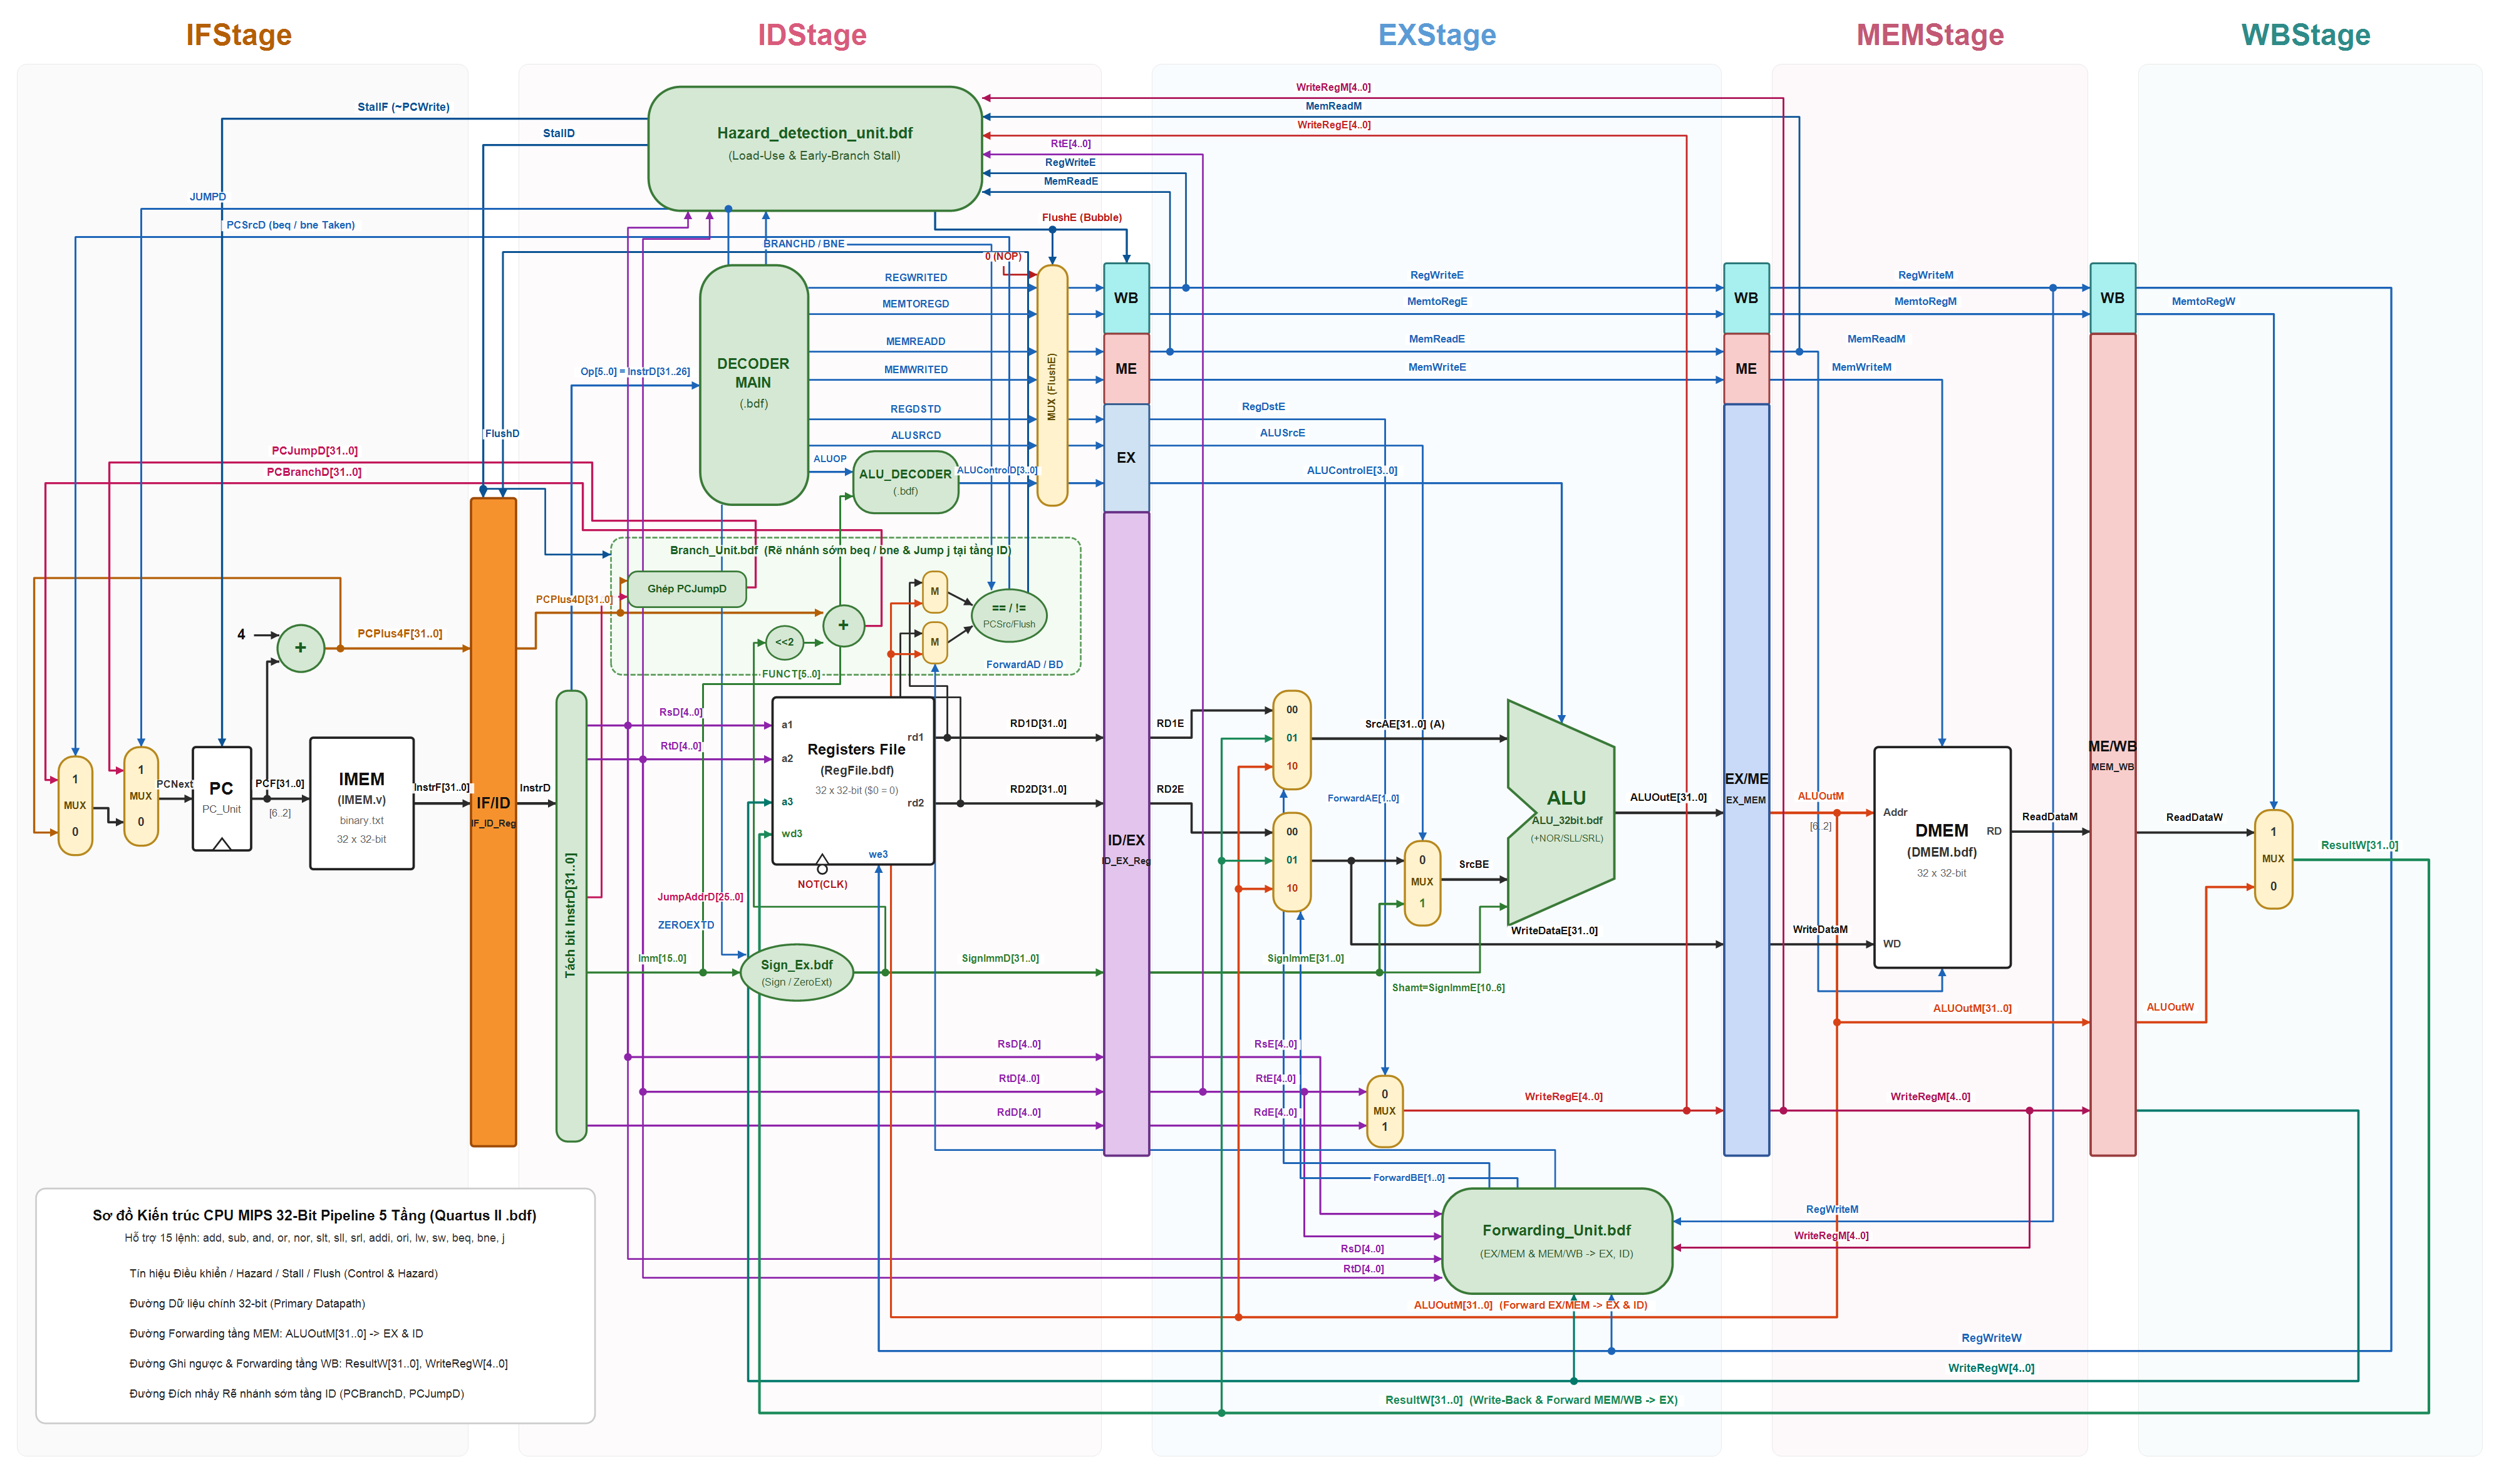
\includegraphics[width=1.18\textwidth]{MIPS_32bit_Pipeline_CPU.png}%
    }
    \caption{Sơ đồ khối tổng quát kiến trúc CPU MIPS 32-bit Pipeline 5 tầng (\texttt{IF, ID, EX, MEM, WB}) tích hợp khối Forwarding Unit và Hazard Detection Unit}
    \label{fig:cpu_datapath_control}
\end{figure}

\subsection{Tầng 1: Khối Nạp lệnh -- Instruction Fetch (\texttt{IF}) và Thanh ghi \texttt{IF\_ID\_Reg}}
Tại tầng \texttt{IF}, thanh ghi bộ đếm chương trình \texttt{PC} lưu giữ địa chỉ byte 32-bit của lệnh hiện hành \texttt{PCF[31:0]}. Trong mỗi chu kỳ:
\begin{itemize}
    \item \textbf{Truy xuất bộ nhớ lệnh (\texttt{IMEM.v})}: Hệ thống trích 5 bit địa chỉ \texttt{PCF[6:2]} đưa vào cổng \texttt{addr[4:0]} của \texttt{IMEM} để đọc tổ hợp mã lệnh 32-bit \texttt{InstrF[31:0]}.
    \item \textbf{Tăng địa chỉ (\texttt{PC + 4})}: Khối \texttt{Adder\_32bit.bdf} cộng giá trị \texttt{PCF[31:0]} với hằng số $32'\text{d}4$ để tạo địa chỉ lệnh kế tiếp \texttt{PCPlus4F[31:0]}.
    \item \textbf{Mạch chọn địa chỉ \texttt{PCNext[31:0]}}: Hai bộ hợp kênh 32-bit \texttt{MUX32to1.bdf} mắc nối tiếp chọn địa chỉ nạp vào \texttt{PC}:
    \begin{equation}
        \text{PCNext}[31:0] = \begin{cases}
            \text{PCJumpD}[31:0]   & \text{khi } \text{JUMPD} = 1 \\
            \text{PCBranchD}[31:0] & \text{khi } \text{JUMPD} = 0 \text{ và } \text{PCSrcD} = 1 \\
            \text{PCPlus4F}[31:0]  & \text{khi } \text{JUMPD} = 0 \text{ và } \text{PCSrcD} = 0
        \end{cases}
    \end{equation}
    \item \textbf{Thanh ghi chặn tầng \texttt{IF\_ID\_Reg.bdf} (64-bit)}: Chốt $\{\texttt{PCPlus4F[31:0]}, \texttt{InstrF[31:0]}\}$ sang tầng \texttt{ID} khi $\text{StallD} = 0$, hoặc xóa về $32'\text{h}00000000$ (\texttt{nop}) khi $\text{FlushD} = 1$.
\end{itemize}

\subsection{Tầng 2: Khối Giải mã -- Instruction Decode (\texttt{ID}) và Thanh ghi \texttt{ID\_EX\_Reg}}
\begin{enumerate}
    \item \textbf{Đọc và ghi Tập thanh ghi (\texttt{RegFile.bdf})}: Gồm 32 thanh ghi 32-bit (\texttt{\$0}..\texttt{\$31}), có 2 cổng đọc tổ hợp (\texttt{RD1D}, \texttt{RD2D}) và 1 cổng ghi đồng bộ tại \textbf{sườn xuống} của xung nhịp (\texttt{CLK\_N = NOT(CLK)}), trong đó thanh ghi \texttt{\$0} nối cứng \texttt{EN = GND}.
    \item \textbf{Mở rộng bit hằng số 16-bit (\texttt{Sign\_Ex.bdf})}: Với $\text{ext\_bit} = \text{InstrD}[15] \cdot \overline{\text{ZEROEXTD}}$:
    \begin{equation}
        \text{SignImmD}[31:0] = \Big\{ \underbrace{\text{ext\_bit}, \text{ext\_bit}, \dots, \text{ext\_bit}}_{16\text{ bits}}, \ \text{InstrD}[15:0] \Big\}
    \end{equation}
    \item \textbf{Tính địa chỉ và kiểm tra điều kiện rẽ nhánh sớm (\texttt{Branch\_Unit.bdf})}: Đặt bộ cộng $\text{PCBranchD} = \text{PCPlus4D} + \{\text{SignImmD}[29:0], 2'\text{b}00\}$ và bộ so sánh bằng 32-bit ngay tại tầng \texttt{ID}.
\end{enumerate}

\subsection{Tầng 3: Khối Thực thi -- Execute (\texttt{EX}) và Thanh ghi \texttt{EX\_MEM\_Reg}}
Hai bộ hợp kênh 4-sang-1 32-bit điều khiển bởi \texttt{ForwardAE[1:0]} và \texttt{ForwardBE[1:0]} chọn dữ liệu đưa vào \texttt{ALU\_32bit.bdf}. Bộ hợp kênh 5-bit \texttt{mux2\_5bit.v} dùng \texttt{RegDstE} để chọn thanh ghi đích \texttt{WriteRegE[4:0]} giữa \texttt{RtE[4:0]} (\texttt{0}) và \texttt{RdE[4:0]} (\texttt{1}).

\begin{figure}[H]
    \centering
    \makebox[\textwidth][c]{%
    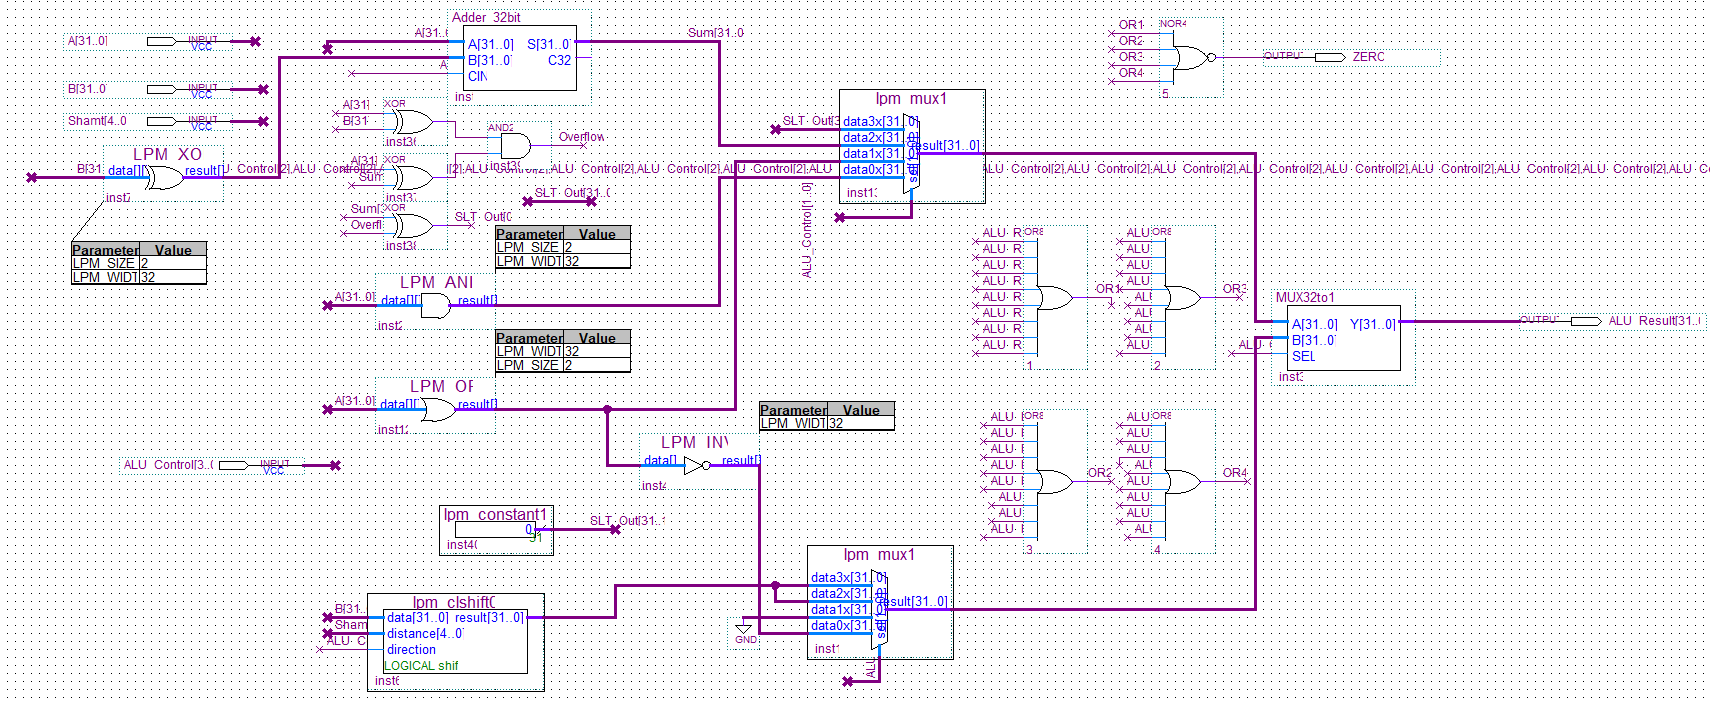
\includegraphics[width=1.05\textwidth]{ALU_32bit_bdf.png}%
    }
    \caption{Sơ đồ nguyên lý khối thực thi số học và luận lý 32-bit (\texttt{ALU\_32bit.bdf}) sử dụng bộ cộng nhìn trước nhớ CLA}
    \label{fig:alu_32bit_schematic}
\end{figure}

\subsection{Tầng 4: Khối Truy xuất Bộ nhớ (\texttt{MEM}) và Tầng 5: Khối Ghi ngược (\texttt{WB})}
Khối \texttt{DMEM.bdf} truy xuất 32 từ nhớ 32-bit theo địa chỉ \texttt{ALUOutM[6:2]}. Tại tầng \texttt{WB}, bộ hợp kênh \texttt{MUX32to1} chọn $\text{ResultW}[31:0] = \text{MemtoRegW} \ ? \ \text{ReadDataW}[31:0] : \text{ALUOutW}[31:0]$ để ghi ngược về \texttt{RegFile}.

\section{Thiết kế Khối Điều khiển Phân cấp (Control Unit) và Bảng Chân trị}

\subsection{Bảng chân trị và Phương trình Boolean của Bộ giải mã chính (\texttt{DECODER\_MAIN.bdf})}
\begin{table}[H]
\centering
\caption{Bảng chân trị các tín hiệu điều khiển của khối giải mã chính (\texttt{DECODER\_MAIN.bdf})}
\label{tab:main_decoder_truth_table}
\setlength{\tabcolsep}{3.5pt}
\makebox[\textwidth][c]{%
\resizebox{1.15\textwidth}{!}{%
\begin{tabular}{@{}lcccccccccccc@{}}
\toprule
\textbf{\shortstack{Nhóm\\lệnh}} & \textbf{\shortstack{Op\\[0pt]{[5:0]}}} & \textbf{\shortstack{REG\\WRITED}} & \textbf{\shortstack{REG\\DSTD}} & \textbf{\shortstack{ALU\\SRCD}} & \textbf{\shortstack{MEM\\READD}} & \textbf{\shortstack{MEM\\WRITED}} & \textbf{\shortstack{MEMTO\\REGD}} & \textbf{\shortstack{BRANCH\\D}} & \textbf{\shortstack{BRANCH\\NED}} & \textbf{\shortstack{JUMP\\D}} & \textbf{\shortstack{ZERO\\EXTD}} & \textbf{\shortstack{ALUOP\\[0pt]{[1:0]}}} \\ \midrule
\textbf{R-Type}        & \texttt{000000} & \textbf{1} & \textbf{1} & 0          & 0          & 0          & 0          & 0          & 0          & 0          & 0          & \textbf{\texttt{10}} \\
\textbf{\texttt{lw}}   & \texttt{100011} & \textbf{1} & 0          & \textbf{1} & \textbf{1} & 0          & \textbf{1} & 0          & 0          & 0          & 0          & \textbf{\texttt{00}} \\
\textbf{\texttt{sw}}   & \texttt{101011} & 0          & 0 (X)      & \textbf{1} & 0          & \textbf{1} & 0 (X)      & 0          & 0          & 0          & 0          & \textbf{\texttt{00}} \\
\textbf{\texttt{beq}}  & \texttt{000100} & 0          & 0 (X)      & 0          & 0          & 0          & 0 (X)      & \textbf{1} & 0          & 0          & 0          & \textbf{\texttt{01}} \\
\textbf{\texttt{bne}}  & \texttt{000101} & 0          & 0 (X)      & 0          & 0          & 0          & 0 (X)      & 0          & \textbf{1} & 0          & 0          & \textbf{\texttt{01}} \\
\textbf{\texttt{addi}} & \texttt{001000} & \textbf{1} & 0          & \textbf{1} & 0          & 0          & 0          & 0          & 0          & 0          & 0          & \textbf{\texttt{00}} \\
\textbf{\texttt{ori}}  & \texttt{001101} & \textbf{1} & 0          & \textbf{1} & 0          & 0          & 0          & 0          & 0          & 0          & \textbf{1} & \textbf{\texttt{11}} \\
\textbf{\texttt{j}}    & \texttt{000010} & 0          & 0 (X)      & 0 (X)      & 0          & 0          & 0 (X)      & 0          & 0          & \textbf{1} & 0          & \texttt{00} (X)      \\ \bottomrule
\end{tabular}%
}%
}
\end{table}
Từ Bảng~\ref{tab:main_decoder_truth_table}, hệ phương trình logic Boolean của khối \texttt{DECODER\_MAIN.bdf} được thiết lập theo phương pháp tổng hợp tổ hợp hai bước dựa trên dạng chuẩn \textbf{Tổng các tích (SOP -- Sum of Products)}:

\begin{align}
    \text{REGWRITED} &= \text{R\_type} + \text{LW} + \text{ADDI} + \text{ORI}, \qquad \text{REGDSTD} = \text{R\_type} \\
    \text{ALUSRCD}   &= \text{LW} + \text{SW} + \text{ADDI} + \text{ORI} \\
    \text{MEMREADD}  &= \text{LW}, \quad \text{MEMWRITED} = \text{SW}, \quad \text{MEMTOREGD} = \text{LW} \\
    \text{BRANCHD}   &= \text{BEQ}, \quad \text{BRANCHNED} = \text{BNE}, \quad \text{JUMPD} = \text{J}, \quad \text{ZEROEXTD} = \text{ORI} \\
    \text{ALUOP}_1   &= \text{R\_type} + \text{ORI}, \quad \text{ALUOP}_0 = \text{BEQ} + \text{BNE} + \text{ORI}
\end{align}

\subsection{Bảng chân trị và Phương trình Boolean của Bộ giải mã ALU (\texttt{ALU\_DECODER.bdf})}
\begin{table}[H]
\centering
\caption{Bảng chân trị giải mã tín hiệu \texttt{ALU\_CONTROLD[3:0]} và ánh xạ kênh MUX trong \texttt{ALU\_32bit.bdf}}
\label{tab:alu_decoder_truth_table}
\setlength{\tabcolsep}{4pt}
\makebox[\textwidth][c]{%
\resizebox{1.15\textwidth}{!}{%
\begin{tabular}{@{}lccccl@{}}
\toprule
\textbf{Nhóm lệnh / Lệnh} & \textbf{\shortstack{ALU\_OP\\[0pt]{[1:0]}}} & \textbf{\shortstack{FUNCT\\[0pt]{[5:0]}}} & \textbf{\shortstack{ALU\_CONTROLD\\[0pt]{[3:0]}}} & \textbf{\shortstack{Kênh MUX\\[0pt]{\{C3,C1,C0\}}}} & \textbf{Phép toán tại \texttt{ALU\_32bit}} \\ \midrule
\texttt{lw}, \texttt{sw}, \texttt{addi} & \texttt{00} & \texttt{XXXXXX} & \textbf{\texttt{0010}} & \texttt{010} (Kênh 2) & Cộng: $A + B$ ($\text{C}_2 = 0$) \\
\texttt{beq}, \texttt{bne}              & \texttt{01} & \texttt{XXXXXX} & \textbf{\texttt{0110}} & \texttt{010} (Kênh 2) & Trừ: $A + \overline{B} + 1$ ($\text{C}_2 = 1$) \\
\texttt{ori}                            & \texttt{11} & \texttt{XXXXXX} & \textbf{\texttt{0001}} & \texttt{001} (Kênh 1) & Hoặc logic: $A \mid B$ \\ \midrule
R-type: \texttt{and}                    & \texttt{10} & \texttt{100100} & \textbf{\texttt{0000}} & \texttt{000} (Kênh 0) & Và logic: $A \ \& \ B$ \\
R-type: \texttt{or}                     & \texttt{10} & \texttt{100101} & \textbf{\texttt{0001}} & \texttt{001} (Kênh 1) & Hoặc logic: $A \mid B$ \\
R-type: \texttt{add}                    & \texttt{10} & \texttt{100000} & \textbf{\texttt{0010}} & \texttt{010} (Kênh 2) & Cộng: $A + B$ ($\text{C}_2 = 0$) \\
R-type: \texttt{sub}                    & \texttt{10} & \texttt{100010} & \textbf{\texttt{0110}} & \texttt{010} (Kênh 2) & Trừ: $A - B$ ($\text{C}_2 = 1$) \\
R-type: \texttt{slt}                    & \texttt{10} & \texttt{101010} & \textbf{\texttt{0111}} & \texttt{011} (Kênh 3) & So sánh có dấu: $S_{31} \oplus \text{Overflow}$ \\
R-type: \texttt{nor}                    & \texttt{10} & \texttt{100111} & \textbf{\texttt{1000}} & \texttt{100} (Kênh 4) & Đảo hoặc: $\sim(A \mid B)$ \\
R-type: \texttt{sll}                    & \texttt{10} & \texttt{000000} & \textbf{\texttt{1010}} & \texttt{110} (Kênh 6) & Dịch trái: $B \ll \text{Shamt}$ ($\text{dir} = \text{C}_0 = 0$) \\
R-type: \texttt{srl}                    & \texttt{10} & \texttt{000010} & \textbf{\texttt{1011}} & \texttt{111} (Kênh 7) & Dịch phải: $B \gg \text{Shamt}$ ($\text{dir} = \text{C}_0 = 1$) \\ \bottomrule
\end{tabular}%
}%
}
\end{table}

Đặt $\text{Is\_R} = \text{ALU\_OP}_1 \cdot \overline{\text{ALU\_OP}_0}$, hệ phương trình Boolean của \texttt{ALU\_CONTROLD[3:0]} là:
\begin{align}
    \text{ALU\_CONTROLD}_3 &= \text{Is\_R} \cdot \left( \overline{\text{FUNCT}_5} + \text{FUNCT}_2 \cdot \text{FUNCT}_1 \right) \\
    \text{ALU\_CONTROLD}_2 &= \left(\overline{\text{ALU\_OP}_1} \cdot \text{ALU\_OP}_0\right) + \left(\text{Is\_R} \cdot \text{FUNCT}_5 \cdot \overline{\text{FUNCT}_2} \cdot \text{FUNCT}_1\right) \\
    \text{ALU\_CONTROLD}_1 &= \overline{\text{ALU\_OP}_1} + \left(\text{Is\_R} \cdot \overline{\text{FUNCT}_2}\right) \\
    \text{ALU\_CONTROLD}_0 &= \left(\text{ALU\_OP}_1 \cdot \text{ALU\_OP}_0\right) \nonumber \\
                           &\quad + \text{Is\_R} \cdot \left( \text{FUNCT}_3 + \overline{\text{FUNCT}_1}\cdot\text{FUNCT}_0 + \overline{\text{FUNCT}_5}\cdot\text{FUNCT}_1 \right)
\end{align}

\begin{figure}[H]
    \centering
    \begin{subfigure}[b]{\textwidth}
        \centering
        \makebox[\textwidth][c]{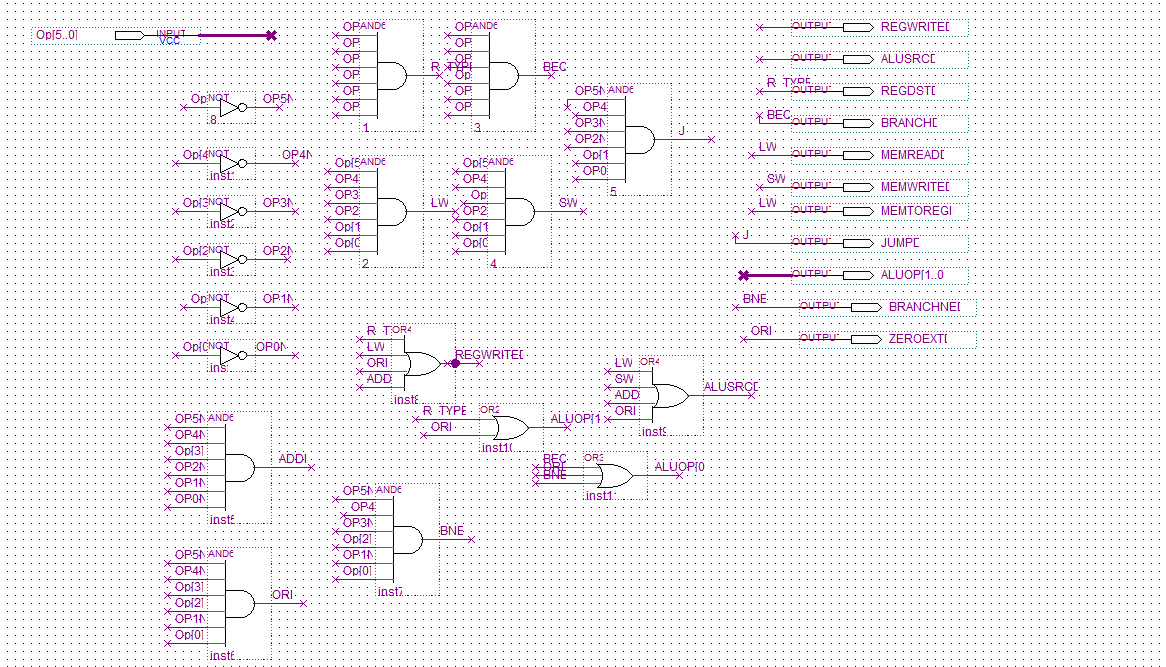
\includegraphics[width=1.12\textwidth]{decoder_main.png}}
        \caption{Khối giải mã chính (\texttt{DECODER\_MAIN.bdf})}
        \label{fig:decoder_main_sub}
    \end{subfigure}
    
    \vspace{0.4cm} % Khoảng cách giữa 2 hình
    
    \begin{subfigure}[b]{\textwidth}
        \centering
        \makebox[\textwidth][c]{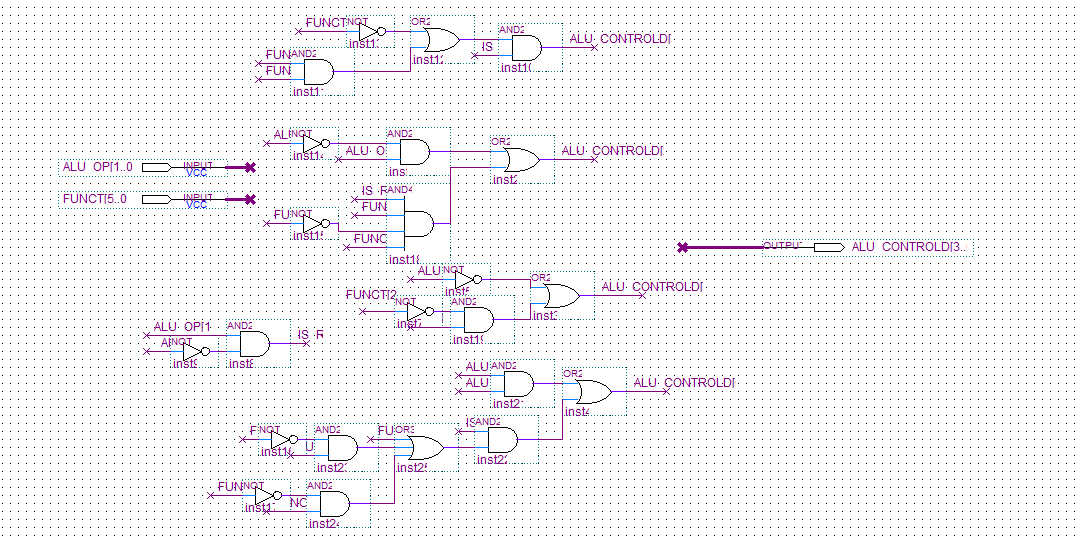
\includegraphics[width=1.12\textwidth]{alu_decoder.png}}
        \caption{Khối giải mã ALU (\texttt{ALU\_DECODER.bdf})}
        \label{fig:alu_decoder_sub}
    \end{subfigure}
    \caption{Sơ đồ mạch logic tổ hợp của khối giải mã chính (\texttt{DECODER\_MAIN.bdf}) và khối giải mã ALU (\texttt{ALU\_DECODER.bdf})}
    \label{fig:control_unit_schematic}
\end{figure}


\section{Biểu thức Logic Boolean của Khối Forwarding Unit và Hazard Detection Unit}

\subsection{Biểu thức Logic Boolean của Khối Chuyển tiếp Dữ liệu (\texttt{Forwarding\_Unit.bdf})}
Với $\text{NonZero}(X) = X_4 + X_3 + X_2 + X_1 + X_0$ và $\text{Equal5}(X, Y) = \prod_{i=0}^{4} \overline{X_i \oplus Y_i}$:
Ngăn không cho chuyển tiếp (Forwarding) hay dừng ống lệnh (Stall) đối với thanh ghi \texttt{\$0}; thanh ghi \texttt{\$0} luôn có giá trị cố định bằng $0$.
\begin{align}
    \text{ForwardAE}_1 &= \text{RegWriteM} \cdot \text{NonZero}(\text{WriteRegM}) \cdot \text{Equal5}(\text{WriteRegM}, \text{RsE}) \\
    \text{ForwardAE}_0 &= \text{RegWriteW} \cdot \text{NonZero}(\text{WriteRegW}) \cdot \text{Equal5}(\text{WriteRegW}, \text{RsE}) \cdot \overline{\text{ForwardAE}_1} \\
    \text{ForwardBE}_1 &= \text{RegWriteM} \cdot \text{NonZero}(\text{WriteRegM}) \cdot \text{Equal5}(\text{WriteRegM}, \text{RtE}) \\
    \text{ForwardBE}_0 &= \text{RegWriteW} \cdot \text{NonZero}(\text{WriteRegW}) \cdot \text{Equal5}(\text{WriteRegW}, \text{RtE}) \cdot \overline{\text{ForwardBE}_1} \\
    \text{ForwardAD}   &= \text{RegWriteM} \cdot \text{NonZero}(\text{WriteRegM}) \cdot \text{Equal5}(\text{WriteRegM}, \text{RsD}) \\
    \text{ForwardBD}   &= \text{RegWriteM} \cdot \text{NonZero}(\text{WriteRegM}) \cdot \text{Equal5}(\text{WriteRegM}, \text{RtD})
\end{align}

\begin{figure}[H]
    \centering
    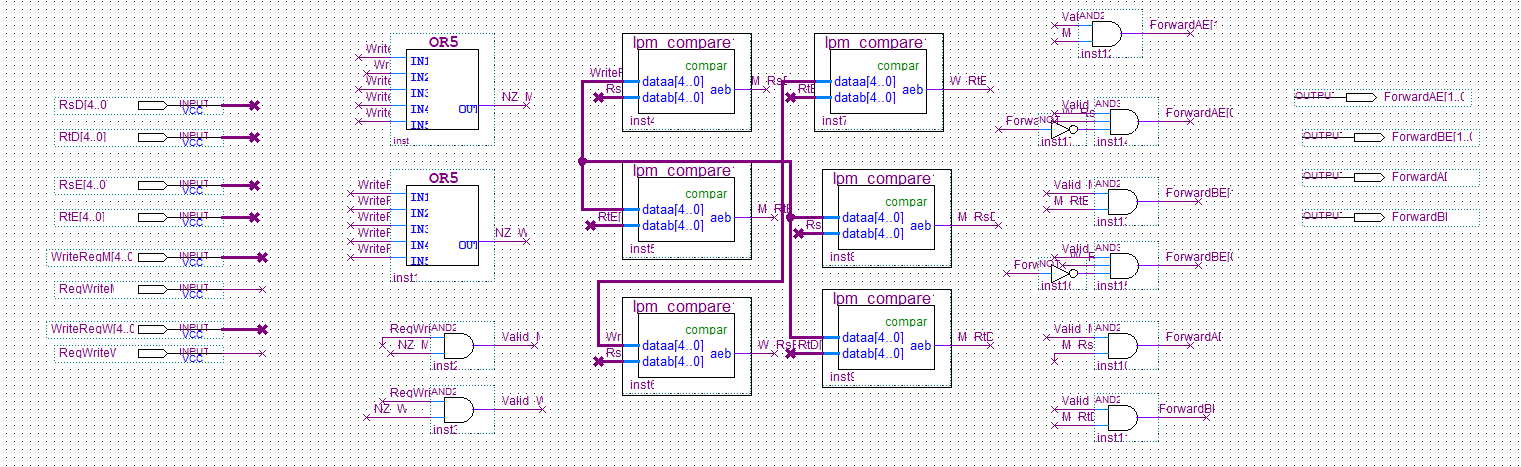
\includegraphics[width=1.0\textwidth]{Forwarding_Unit_bdf.png}
    \caption{Sơ đồ nguyên lý khối chuyển tiếp dữ liệu (\texttt{Forwarding\_Unit.bdf}) xử lý xung đột RAW tại tầng \texttt{EX} và tầng \texttt{ID}}
    \label{fig:forwarding_unit_schematic}
\end{figure}

\subsection{Biểu thức Logic Boolean của Khối Phát hiện Xung đột (\texttt{Hazard\_detection\_unit.bdf}) \& \texttt{Branch\_Unit.bdf}}
\begin{align}
    \text{lw\_stall} &= \text{MemReadE} \cdot \text{NonZero}(\text{RtE}) \cdot \Big( \text{Equal5}(\text{RtE}, \text{RsD}) + \text{Equal5}(\text{RtE}, \text{RtD}) \Big) \\
    \text{br\_ex\_stall} &= \text{AnyBranchD} \cdot \text{RegWriteE} \cdot \text{NonZero}(\text{WriteRegE}) \nonumber \\
                         &\quad \cdot \Big( \text{Equal5}(\text{WriteRegE}, \text{RsD}) + \text{Equal5}(\text{WriteRegE}, \text{RtD}) \Big) \\
    \text{br\_mem\_stall} &= \text{AnyBranchD} \cdot \text{MemReadM} \cdot \text{NonZero}(\text{WriteRegM}) \nonumber \\
                          &\quad \cdot \Big( \text{Equal5}(\text{WriteRegM}, \text{RsD}) + \text{Equal5}(\text{WriteRegM}, \text{RtD}) \Big) \\
    \text{StallF} &= \text{StallD} = \text{FlushE} = \text{lw\_stall} + \text{br\_ex\_stall} + \text{br\_mem\_stall} \\
    \text{PCSrcD} &= \Big( (\text{BRANCHD} \cdot \text{EqualID}) + (\text{BRANCHNED} \cdot \overline{\text{EqualID}}) \Big) \cdot \overline{\text{StallD}} \\
    \text{FlushD} &= \left( \text{PCSrcD} + \text{JUMPD} \right) \cdot \overline{\text{StallD}}
\end{align}

\begin{figure}[H]
    \centering
    \makebox[\textwidth][c]{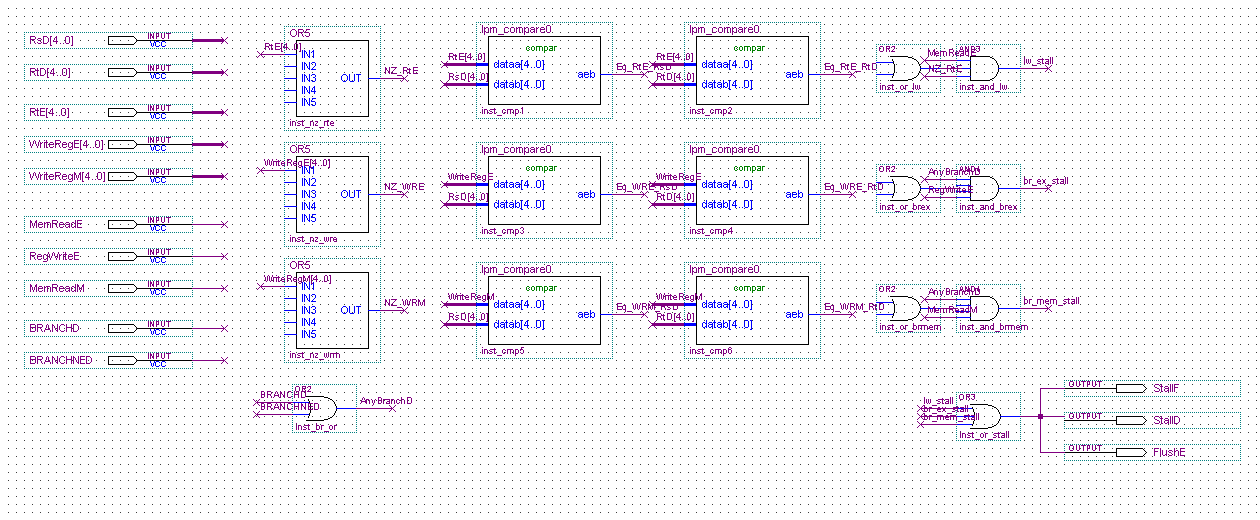
\includegraphics[width=1.10\textwidth]{Hazard_detection_unit_bdf.png}}
    \caption{Sơ đồ nguyên lý khối phát hiện xung đột (\texttt{Hazard\_detection\_unit.bdf})}
    \label{fig:hazard_detection_schematic}
\end{figure}

\begin{figure}[H]
    \centering
    \makebox[\textwidth][c]{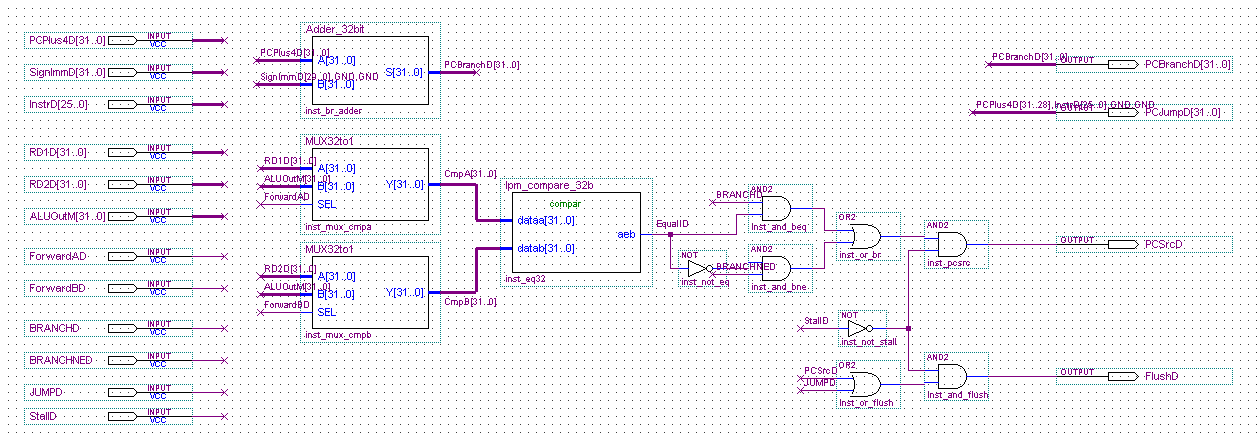
\includegraphics[width=1.10\textwidth]{Branch_Unit_bdf.png}}
    \caption{Sơ đồ nguyên lý khối xử lý rẽ nhánh sớm (\texttt{Branch\_Unit.bdf})}
    \label{fig:branch_unit_schematic}
\end{figure}
% ==============================================================================
% CHƯƠNG 3: HIỆN THỰC HÓA MẠCH & MÔ PHỎNG KIỂM CHỨNG TRÊN QUARTUS II (YÊU CẦU 2)
% ==============================================================================
\chapter{Hiện Thực Mạch và Mô Phỏng Kiểm Tra Trên Quartus II}

\section{Tổ chức Phân cấp Các Module Con và Sơ đồ Kết nối Mức Đỉnh (Top-Level Schematic)}

Hệ thống CPU MIPS 32-bit Pipeline 5 tầng được hiện thực hóa theo phương pháp thiết kế lai (\textit{Hybrid Schematic \& HDL Design}): toàn bộ đường truyền dữ liệu (Datapath), khối điều khiển (Control Unit), bộ cộng nhanh CLA và các khối xử lý xung đột được vẽ trực quan bằng sơ đồ nguyên lý mức cổng (\texttt{.bdf}); trong khi bộ nhớ lệnh \texttt{IMEM.v} và các thanh ghi cơ sở có xóa/cho phép đồng bộ (\texttt{ff\_*.v}) được mô tả bằng Verilog HDL.

\begin{lstlisting}[style=verilogstyle, caption={Mô tả bộ nhớ lệnh IMEM.v tự động nạp mã máy từ file binary.txt}, label={lst:imem}]
module IMEM (
    input  wire [4:0]  addr,   // Nhan PCF[6..2] (Word-aligned address)
    output wire [31:0] q       // Xuat ma may 32-bit InstrF[31..0]
);
    reg [31:0] rom [0:31];

    initial begin
        $readmemb("binary.txt", rom);
    end

    assign q = rom[addr];
endmodule
\end{lstlisting}

\begin{table}[H]
\centering
\caption{Bảng phân cấp chức năng các module thành phần trong dự án \texttt{MIPS\_32BIT\_PIPELINE}}
\label{tab:module_hierarchy}
\resizebox{\textwidth}{!}{%
\begin{tabular}{@{}llcl@{}}
\toprule
\textbf{Miền chức năng} & \textbf{Tên file module} & \textbf{Loại file} & \textbf{Vai trò và đặc điểm kỹ thuật trong hệ thống} \\ \midrule
\multirow{4}{*}{\textbf{1. Tầng IF}}
 & \texttt{ff\_32bit\_en\_sclr.v} & Verilog & Thanh ghi bộ đếm chương trình \texttt{PC} 32-bit, chốt ở sườn lên \texttt{CLK} khi $\text{PC\_En} = \overline{\text{StallF}} + \text{Reset} = 1$. \\
 & \texttt{IMEM.v} & Verilog & Bộ nhớ lệnh ROM $32 \times 32$-bit, đọc tổ hợp mã lệnh \texttt{InstrF[31:0]} tại địa chỉ từ \texttt{PCF[6:2]} qua hàm \texttt{\$readmemb}. \\
 & \texttt{lpm\_constant0.v} & IP/Verilog & Tạo hằng số cố định $32'\text{d}4$ cấp cho bộ cộng địa chỉ tuần tự $\text{PCPlus4F} = \text{PCF} + 4$. \\
 & \texttt{MUX32to1.bdf} & Schematic & Hai bộ hợp kênh 2-sang-1 32-bit nối tiếp chọn địa chỉ \texttt{PCNext[31:0]} theo cờ \texttt{PCSrcD} và \texttt{JUMPD}. \\ \midrule
\multirow{5}{*}{\textbf{2. Tầng ID}}
 & \texttt{DECODER\_MAIN.bdf} & Schematic & Giải mã 6 bit \texttt{Op[5:0]} thành 12 tín hiệu điều khiển đường ống và mã \texttt{ALUOP[1:0]}. \\
 & \texttt{ALU\_DECODER.bdf} & Schematic & Giải mã \texttt{ALUOP[1:0]} và \texttt{FUNCT[5:0]} thành mã điều khiển 4-bit \texttt{ALU\_CONTROLD[3:0]}. \\
 & \texttt{RegFile.bdf} & Schematic & Tập 32 thanh ghi 32-bit (\texttt{\$0} khóa cứng \texttt{EN = GND}), đọc tổ hợp 2 cổng, ghi đồng bộ ở sườn xuống \texttt{CLK\_N}. \\
 & \texttt{Sign\_Ex.bdf} & Schematic & Mở rộng hằng số 16-bit lên 32-bit có dấu (\texttt{ZEROEXTD = 0}) hoặc không dấu (\texttt{ZEROEXTD = 1} cho \texttt{ori}). \\
 & \texttt{Branch\_Unit.bdf} & Schematic & Tính sẵn \texttt{PCBranchD}, \texttt{PCJumpD}, so sánh bằng 32-bit (\texttt{EqualID}) tại tầng \texttt{ID} và phát cờ \texttt{PCSrcD}, \texttt{FlushD}. \\ \midrule
\multirow{4}{*}{\textbf{3. Tầng EX}}
 & \texttt{lpm\_mux1.v} & IP/Verilog & Hai bộ hợp kênh 4-sang-1 32-bit chọn toán hạng đầu vào ALU theo mã \texttt{ForwardAE[1:0]} và \texttt{ForwardBE[1:0]}. \\
 & \texttt{ALU\_32bit.bdf} & Schematic & Khối thực thi trung tâm: tích hợp bộ cộng/trừ CLA 32-bit, cổng \texttt{AND/OR/NOR}, bộ dịch \texttt{lpm\_clshift0} và mạch \texttt{SLT}. \\
 & \texttt{Adder\_32bit.bdf} & Schematic & Bộ cộng nhìn trước nhớ phân cấp 32-bit ghép từ \texttt{CLA\_16bit.bdf}, \texttt{LCU\_16bit.bdf}, \texttt{CLA\_4bit.bdf} và \texttt{FA\_1b.bdf}. \\
 & \texttt{mux2\_5bit.v} & Verilog & Bộ hợp kênh 2-sang-1 5-bit chọn thanh ghi đích \texttt{WriteRegE[4:0]} giữa \texttt{RtE[4:0]} (\texttt{0}) và \texttt{RdE[4:0]} (\texttt{1}). \\ \midrule
\textbf{4. Tầng MEM \& WB}
 & \texttt{DMEM.bdf} & Schematic & Bộ nhớ dữ liệu RAM $32 \times 32$-bit truy xuất theo địa chỉ từ \texttt{ALUOutM[6:2]}, ghi ở sườn lên \texttt{CLK} khi \texttt{MemWriteM = 1}. \\ \midrule
\multirow{4}{*}{\textbf{5. Thanh ghi Tầng}}
 & \texttt{IF\_ID\_Reg.bdf} & Schematic & Thanh ghi chặn tầng \texttt{IF/ID} (64-bit): có chân giữ \texttt{StallD} và xóa đồng bộ \texttt{FlushD}. \\
 & \texttt{ID\_EX\_Reg.bdf} & Schematic & Thanh ghi chặn tầng \texttt{ID/EX} (121-bit): chuyển 10 bit Control + 111 bit Datapath; xóa về \texttt{NOP} khi \texttt{FlushE = 1}. \\
 & \texttt{EX\_MEM\_Reg.bdf} & Schematic & Thanh ghi chặn tầng \texttt{EX/MEM} (73-bit): chuyển 4 bit Control + \texttt{ALUOutM}, \texttt{WriteDataM}, \texttt{WriteRegM}. \\
 & \texttt{MEM\_WB\_Reg.bdf} & Schematic & Thanh ghi chặn tầng \texttt{MEM/WB} (71-bit): chuyển 2 bit Control + \texttt{ReadDataW}, \texttt{ALUOutW}, \texttt{WriteRegW}. \\ \midrule
\multirow{2}{*}{\textbf{6. Khối Hazard}}
 & \texttt{Forwarding\_Unit.bdf} & Schematic & Phát hiện xung đột RAW và xuất tín hiệu điều khiển \texttt{ForwardAE[1:0]}, \texttt{ForwardBE[1:0]}, \texttt{ForwardAD}, \texttt{ForwardBD}. \\
 & \texttt{Hazard\_detection\_unit.bdf} & Schematic & Phát hiện xung đột \texttt{Load-Use}, \texttt{ALU-Branch}, \texttt{Load-Branch} để kích hoạt \texttt{StallF}, \texttt{StallD} và \texttt{FlushE}. \\ \bottomrule
\end{tabular}%
}
\end{table}

\begin{figure}[H]
    \noindent\hspace*{-0.5cm}\makebox[\textwidth][c]{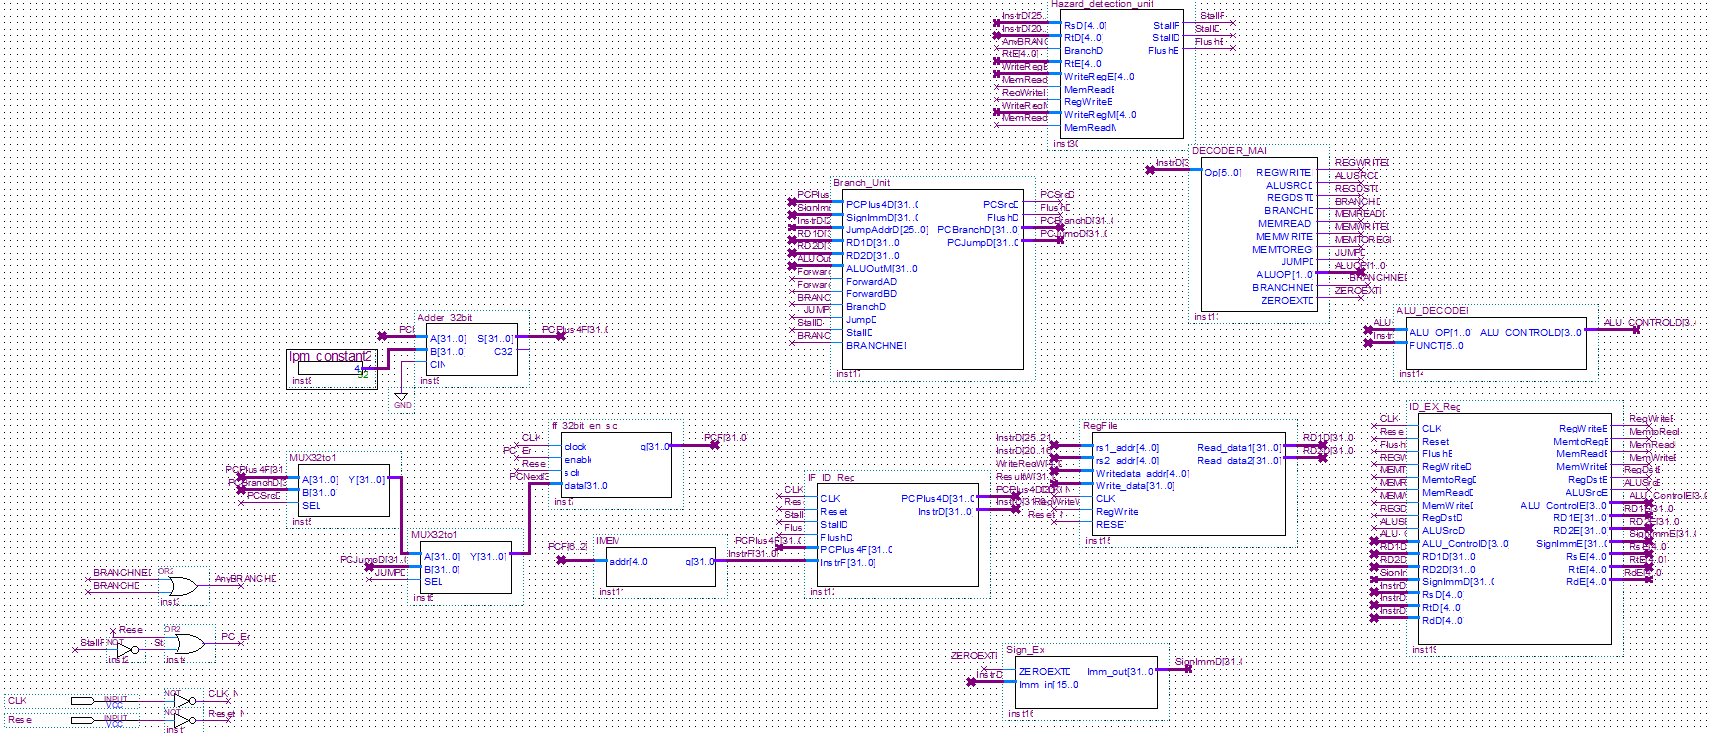
\includegraphics[width=19cm]{top_left.png}}
    \caption{Sơ đồ nguyên lý mức đỉnh (\texttt{MIPS\_32BIT\_PIPELINE.bdf}) -- Nửa trái: Tầng \texttt{IF}, tầng \texttt{ID}, \texttt{Control Unit} và \texttt{Hazard\_detection\_unit}}
    \label{fig:top_level_bdf_left}
\end{figure}

\begin{figure}[H]
    \noindent\hspace*{-0.5cm}\makebox[\textwidth][c]{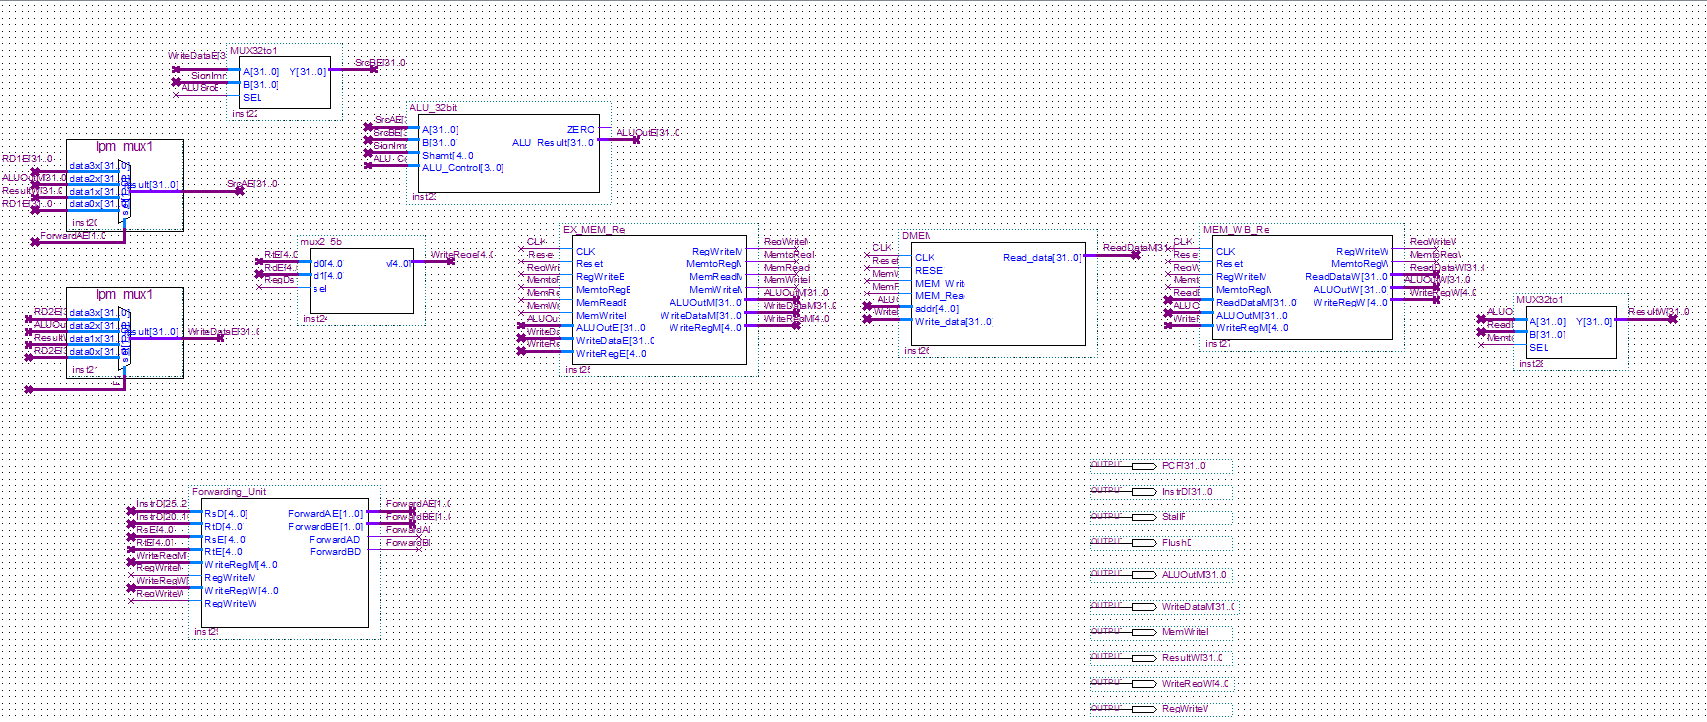
\includegraphics[width=19cm]{top_right.png}}
    \caption{Sơ đồ nguyên lý mức đỉnh (\texttt{MIPS\_32BIT\_PIPELINE.bdf}) -- Nửa phải: Tầng \texttt{EX}, \texttt{Forwarding\_Unit}, tầng \texttt{MEM}, tầng \texttt{WB} và các chân Output}
    \label{fig:top_level_bdf_right}
\end{figure}
\section{Xây dựng Chương trình Hợp ngữ Kiểm thử Toàn diện và Bảng Mã Máy 32-Bit}

\begin{table}[H]
\centering
\caption{Bảng chương trình hợp ngữ kiểm thử toàn diện 27 lệnh và mã máy 32-bit (Hex/Binary) nạp vào \texttt{IMEM}}
\label{tab:benchmark_machine_code}
\resizebox{\textwidth}{!}{%
\begin{tabular}{@{}ccllcccl@{}}
\toprule
\textbf{TT} & \textbf{Địa chỉ} & \textbf{Nhãn} & \textbf{Câu lệnh Assembly} & \textbf{Mã máy Hex} & \textbf{Mã nhị phân 32-bit (\texttt{Op\_Rs\_Rt\_Rd\_Shamt\_Funct / Imm})} & \textbf{Mục đích kiểm chứng phần cứng} \\ \midrule
\texttt{I0}  & \texttt{0x00} & \texttt{main:}   & \texttt{addi \$1, \$0, 5}      & \texttt{0x20010005} & \texttt{001000\_00000\_00001\_0000000000000101} & Khởi tạo $\texttt{\$1} = 5$ \\
\texttt{I1}  & \texttt{0x04} &                  & \texttt{addi \$1, \$1, 7}      & \texttt{0x20210007} & \texttt{001000\_00001\_00001\_0000000000000111} & Forward \texttt{EX/MEM} (\texttt{ForwardAE=10}): $\texttt{\$1} = 5+7 = 12$ \\
\texttt{I2}  & \texttt{0x08} &                  & \texttt{addi \$1, \$1, 3}      & \texttt{0x20210003} & \texttt{001000\_00001\_00001\_0000000000000011} & \textbf{Double Data Hazard} trên \texttt{\$1}: $\texttt{\$1} = 12+3 = 15$ (\texttt{0x0F}) \\ \midrule
\texttt{I3}  & \texttt{0x0C} &                  & \texttt{addi \$2, \$0, -4}     & \texttt{0x2002FFFC} & \texttt{001000\_00000\_00010\_1111111111111100} & Mở rộng dấu âm (\texttt{Sign\_Ex}): $\texttt{\$2} = -4$ (\texttt{0xFFFFFFFC}) \\
\texttt{I4}  & \texttt{0x10} &                  & \texttt{slt \$3, \$2, \$1}     & \texttt{0x0041182A} & \texttt{000000\_00010\_00001\_00011\_00000\_101010} & So sánh có dấu $(-4 < 15)$: $\texttt{\$3} = 1$ \\
\texttt{I5}  & \texttt{0x14} &                  & \texttt{sll \$4, \$3, 4}       & \texttt{0x00032100} & \texttt{000000\_00000\_00011\_00100\_00100\_000000} & Dịch trái logic $1 \ll 4$: $\texttt{\$4} = 16$ (\texttt{0x10}) \\
\texttt{I6}  & \texttt{0x18} &                  & \texttt{ori \$4, \$4, 5}       & \texttt{0x34840005} & \texttt{001101\_00100\_00100\_0000000000000101} & Mở rộng \texttt{0} (\texttt{ZEROEXTD=1}): $\texttt{\$4} = 16 \mid 5 = 21$ (\texttt{0x15}) \\
\texttt{I7}  & \texttt{0x1C} &                  & \texttt{srl \$4, \$4, 1}       & \texttt{0x00042042} & \texttt{000000\_00000\_00100\_00100\_00001\_000010} & Dịch phải logic $21 \gg 1$: $\texttt{\$4} = 10$ (\texttt{0x0A}) \\
\texttt{I8}  & \texttt{0x20} &                  & \texttt{sub \$5, \$1, \$4}     & \texttt{0x00242822} & \texttt{000000\_00001\_00100\_00101\_00000\_100010} & Phép trừ CLA 32-bit: $\texttt{\$5} = 15 - 10 = 5$ \\
\texttt{I9}  & \texttt{0x24} &                  & \texttt{and \$6, \$1, \$4}     & \texttt{0x00243024} & \texttt{000000\_00001\_00100\_00110\_00000\_100100} & Phép AND bitwise: $\texttt{\$6} = 15 \ \& \ 10 = 10$ (\texttt{0x0A}) \\
\texttt{I10} & \texttt{0x28} &                  & \texttt{or \$0, \$1, \$4}      & \texttt{0x00240025} & \texttt{000000\_00001\_00100\_00000\_00000\_100101} & \textbf{Bẫy ghi vào \texttt{\$0}}: Cố ghi $15$ vào \texttt{\$0} ($\texttt{\$0}$ vẫn $= 0$) \\
\texttt{I11} & \texttt{0x2C} &                  & \texttt{nor \$2, \$0, \$0}     & \texttt{0x00001027} & \texttt{000000\_00000\_00000\_00010\_00000\_100111} & Kiểm chứng chặn Forward \texttt{\$0}: $\texttt{\$2} = \sim(0 \mid 0) = \texttt{0xFFFFFFFF}$ \\
\texttt{I12} & \texttt{0x30} &                  & \texttt{add \$5, \$5, \$2}     & \texttt{0x00A22820} & \texttt{000000\_00101\_00010\_00101\_00000\_100000} & Cộng số âm: $\texttt{\$5} = 5 + (-1) = 4$ \\ \midrule
\texttt{I13} & \texttt{0x34} &                  & \texttt{sw \$1, 8(\$0)}        & \texttt{0xAC010008} & \texttt{101011\_00000\_00001\_0000000000001000} & Ghi RAM (\texttt{MemWriteM=1}): $\text{DMEM}[2] \leftarrow 15$ (\texttt{0x0F}) \\
\texttt{I14} & \texttt{0x38} &                  & \texttt{lw \$6, 8(\$0)}        & \texttt{0x8C060008} & \texttt{100011\_00000\_00110\_0000000000001000} & Đọc RAM: $\texttt{\$6} \leftarrow \text{DMEM}[2] = 15$ (\texttt{0x0F}) \\
\texttt{I15} & \texttt{0x3C} &                  & \texttt{add \$7, \$6, \$5}     & \texttt{0x00C53820} & \texttt{000000\_00110\_00101\_00111\_00000\_100000} & \textbf{Load-Use Stall 1 nhịp} + Forward \texttt{WB}: $\texttt{\$7} = 15+4 = 19$ (\texttt{0x13}) \\ \midrule
\texttt{I16} & \texttt{0x40} &                  & \texttt{beq \$7, \$5, trap1}   & \texttt{0x10E50001} & \texttt{000100\_00111\_00101\_0000000000000001} & \textbf{ALU-Branch Stall 1 nhịp} + \texttt{ForwardAD}: $19 \neq 4 \rightarrow$ Không nhảy \\
\texttt{I17} & \texttt{0x44} &                  & \texttt{beq \$6, \$1, br1\_ok} & \texttt{0x10C10001} & \texttt{000100\_00110\_00001\_0000000000000001} & $15 == 15 \rightarrow$ \textbf{Nhảy (\texttt{FlushD=1})}, xóa lệnh \texttt{trap1} \\
\texttt{I18} & \texttt{0x48} & \texttt{trap1:}  & \texttt{addi \$7, \$0, 99}     & \texttt{0x20070063} & \texttt{001000\_00000\_00111\_0000000001100011} & \textit{(Lệnh bẫy 1 -- Bị \texttt{FlushD} xóa thành \texttt{NOP})} \\ \midrule
\texttt{I19} & \texttt{0x4C} & \texttt{br1\_ok:}& \texttt{lw \$3, 8(\$0)}        & \texttt{0x8C030008} & \texttt{100011\_00000\_00011\_0000000000001000} & Đọc RAM: $\texttt{\$3} \leftarrow 15$ (\texttt{0x0F}) \\
\texttt{I20} & \texttt{0x50} &                  & \texttt{bne \$3, \$1, trap2}  & \texttt{0x14610001} & \texttt{000101\_00011\_00001\_0000000000000001} & \textbf{Load-Branch Stall 2 nhịp}; $15 \neq 15$ (Sai) $\rightarrow$ Không nhảy \\
\texttt{I21} & \texttt{0x54} &                  & \texttt{bne \$3, \$5, br2\_ok} & \texttt{0x14650001} & \texttt{000101\_00011\_00101\_0000000000000001} & $15 \neq 4 \rightarrow$ \textbf{Nhảy (\texttt{FlushD=1})}, xóa lệnh \texttt{trap2} \\
\texttt{I22} & \texttt{0x58} & \texttt{trap2:}  & \texttt{addi \$3, \$0, 88}     & \texttt{0x20030058} & \texttt{001000\_00000\_00011\_0000000001011000} & \textit{(Lệnh bẫy 2 -- Bị \texttt{FlushD} xóa thành \texttt{NOP})} \\ \midrule
\texttt{I23} & \texttt{0x5C} & \texttt{br2\_ok:}& \texttt{j finish}              & \texttt{0x08000019} & \texttt{000010\_00000000000000000000011001}     & \textbf{Nhảy \texttt{j} (\texttt{FlushD=1})} tới \texttt{0x64}, xóa lệnh \texttt{trap3} \\
\texttt{I24} & \texttt{0x60} & \texttt{trap3:}  & \texttt{addi \$5, \$0, 77}     & \texttt{0x2005004D} & \texttt{001000\_00000\_00101\_0000000001001101} & \textit{(Lệnh bẫy 3 -- Bị \texttt{FlushD} xóa thành \texttt{NOP})} \\
\texttt{I25} & \texttt{0x64} & \texttt{finish:} & \texttt{addi \$2, \$7, 1}      & \texttt{0x20E20001} & \texttt{001000\_00111\_00010\_0000000000000001} & Kết quả chốt hạ: $\texttt{\$2} = 19 + 1 = 20$ (\texttt{0x14}) \\
\texttt{I26} & \texttt{0x68} & \texttt{halt:}   & \texttt{j halt}                & \texttt{0x0800001A} & \texttt{000010\_00000000000000000000011010}     & Khóa \texttt{PC} tại địa chỉ \texttt{0x68} khi hoàn thành \\ \bottomrule
\end{tabular}%
}
\end{table}
\newpage

\section{Phân tích Chi tiết Kết quả Mô phỏng Dạng sóng (Waveform Analysis)}

\begin{figure}[H]
    \noindent\hspace*{-0.5cm}\makebox[\textwidth][c]{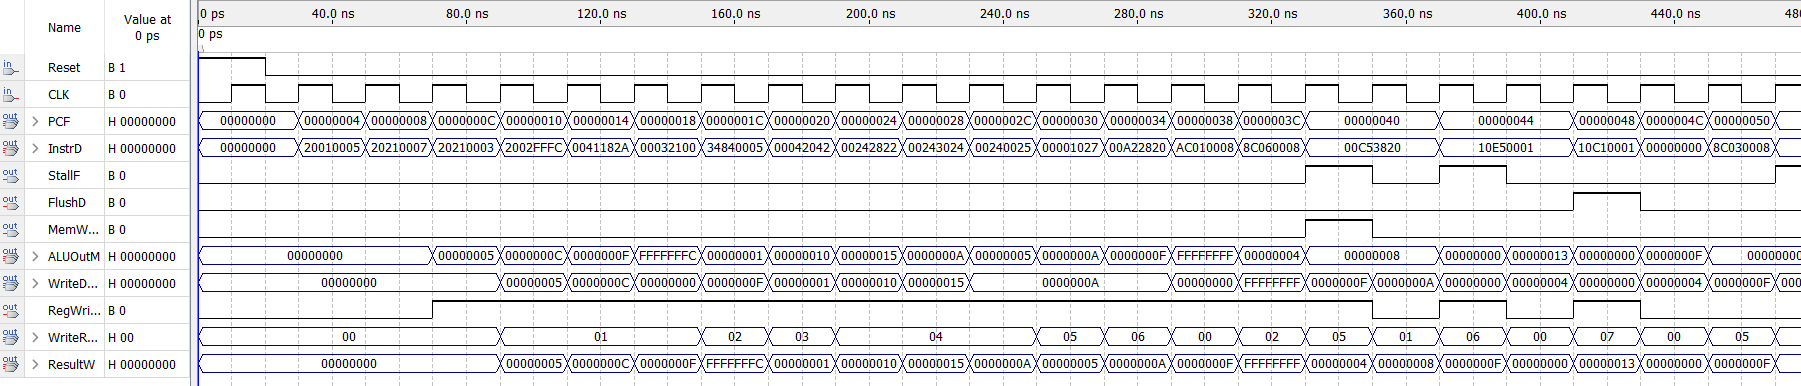
\includegraphics[width=19.8cm, height=6.5cm]{waveform_0_470.png}}
    \caption{Dạng sóng mô phỏng thực tế trên Quartus II từ $0\text{ ns}$ đến $470\text{ ns}$ kiểm chứng luồng lệnh 5 tầng, Forwarding, bảo vệ \texttt{\$0}, Load-Use Stall và Control Hazard}
    \label{fig:waveform_part1}
\end{figure}

\begin{figure}[H]
    \noindent\hspace*{-0.5cm}\makebox[\textwidth][c]{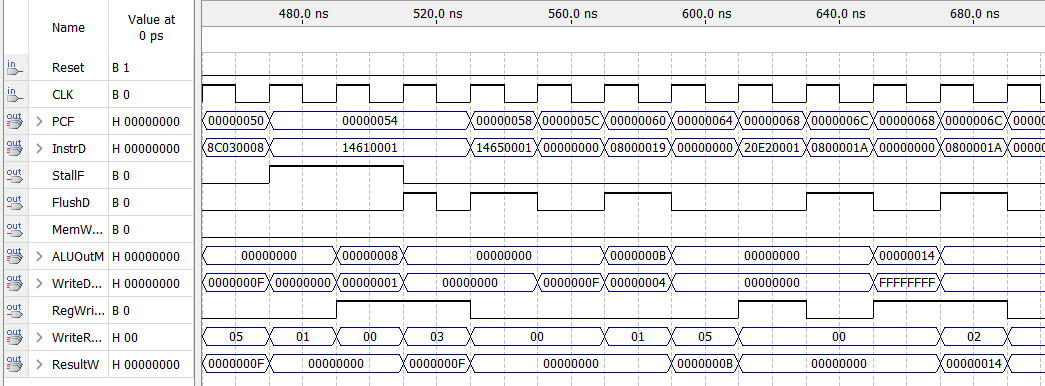
\includegraphics[width=19.8cm, height=6.5cm]{waveform_450_700.png}}
    \caption{Dạng sóng mô phỏng giai đoạn $450\text{--}700\text{ ns}$ minh họa Stall kép 2 chu kỳ (\texttt{lw} $\rightarrow$ \texttt{bne}), lệnh \texttt{bne} nhảy (\texttt{FlushD = 1}), nhảy không điều kiện (\texttt{j finish}) và kết quả chốt cuối cùng $\texttt{\$2} = \texttt{0x00000014}$ ($20$)}
    \label{fig:waveform_part2}
\end{figure}

\newpage

\begin{table}[H]
\centering
\caption{Bảng phân tích đối chiếu giá trị các tín hiệu trên Waveform theo từng chu kỳ xung nhịp ($0\text{--}690\text{ ns}$)}
\label{tab:waveform_cycle_trace}
\setlength{\tabcolsep}{3.5pt}
\renewcommand{\arraystretch}{1.05}
\noindent\hspace*{-0.5cm}\makebox[\textwidth][c]{%
\resizebox{19.4cm}{!}{%
\begin{tabular}{@{}ccccccccccl@{}}
\toprule
\textbf{\shortstack{Chu\\kỳ}} & \textbf{\shortstack{Thời gian\\(ns)}} & \textbf{\texttt{PCF}} & \textbf{\texttt{InstrD}} & \textbf{\shortstack{Stall\\F}} & \textbf{\shortstack{Flush\\D}} & \textbf{\shortstack{Mem\\WriteM}} & \textbf{\texttt{ALUOutM}} & \textbf{\shortstack{Reg\\WriteW}} & \textbf{\shortstack{\texttt{WriteRegW}\\\texttt{: ResultW}}} & \textbf{Sự kiện Pipeline \& Giải thích kỹ thuật} \\ \midrule
\texttt{CC0}  & \texttt{10--30}   & \texttt{00000000} & \texttt{00000000} & \texttt{0} & \texttt{0} & \texttt{0} & \texttt{00000000} & \texttt{0} & \texttt{00 : 00000000} & \parbox{11.5cm}{\raggedright Khởi tạo \texttt{Reset=1} ($0\text{--}20\text{ ns}$); nạp \texttt{I0} tại \texttt{0x00}} \\
\texttt{CC1}  & \texttt{30--50}   & \texttt{00000004} & \texttt{20010005} & \texttt{0} & \texttt{0} & \texttt{0} & \texttt{00000000} & \texttt{0} & \texttt{00 : 00000000} & \parbox{11.5cm}{\raggedright \texttt{I0} (\texttt{addi \$1,\$0,5}) vào tầng \texttt{ID}; nạp \texttt{I1}} \\
\texttt{CC2}  & \texttt{50--70}   & \texttt{00000008} & \texttt{20210007} & \texttt{0} & \texttt{0} & \texttt{0} & \texttt{00000000} & \texttt{0} & \texttt{00 : 00000000} & \parbox{11.5cm}{\raggedright \texttt{I0} vào \texttt{EX} tính $0+5=5$; \texttt{I1} vào \texttt{ID}} \\
\texttt{CC3}  & \texttt{70--90}   & \texttt{0000000C} & \texttt{20210003} & \texttt{0} & \texttt{0} & \texttt{0} & \textbf{\texttt{00000005}} & \texttt{1} & \texttt{00 : 00000000} & \parbox{11.5cm}{\raggedright \texttt{I0} ở \texttt{MEM}; \textbf{\texttt{ForwardAE=10}} đưa $5$ về \texttt{EX} cho \texttt{I1}} \\
\texttt{CC4}  & \texttt{90--110}  & \texttt{00000010} & \texttt{2002FFFC} & \texttt{0} & \texttt{0} & \texttt{0} & \textbf{\texttt{0000000C}} & \textbf{\texttt{1}} & \textbf{\texttt{01 : 00000005}} & \parbox{11.5cm}{\raggedright \texttt{I0} ghi $\texttt{\$1}=5$; \textbf{Double Hazard}: \texttt{I2} lấy $12$ từ \texttt{MEM}} \\
\texttt{CC5}  & \texttt{110--130} & \texttt{00000014} & \texttt{0041182A} & \texttt{0} & \texttt{0} & \texttt{0} & \textbf{\texttt{0000000F}} & \textbf{\texttt{1}} & \textbf{\texttt{01 : 0000000C}} & \parbox{11.5cm}{\raggedright \texttt{I1} ghi $\texttt{\$1}=12$; \texttt{I2} ở \texttt{MEM} đạt $12+3=15$ (\texttt{0x0F})} \\
\texttt{CC6}  & \texttt{130--150} & \texttt{00000018} & \texttt{00032100} & \texttt{0} & \texttt{0} & \texttt{0} & \textbf{\texttt{FFFFFFFC}} & \textbf{\texttt{1}} & \textbf{\texttt{01 : 0000000F}} & \parbox{11.5cm}{\raggedright \texttt{I2} ghi $\texttt{\$1}=15$; \texttt{I3} ở \texttt{MEM} xuất $-4$ (\texttt{0xFFFFFFFC})} \\
\texttt{CC7}  & \texttt{150--170} & \texttt{0000001C} & \texttt{34840005} & \texttt{0} & \texttt{0} & \texttt{0} & \textbf{\texttt{00000001}} & \textbf{\texttt{1}} & \textbf{\texttt{02 : FFFFFFFC}} & \parbox{11.5cm}{\raggedright \texttt{I3} ghi $\texttt{\$2}=-4$; \texttt{I4} (\texttt{slt}) ở \texttt{MEM} xuất $1$ ($-4 < 15$)} \\
\texttt{CC8}  & \texttt{170--190} & \texttt{00000020} & \texttt{00042042} & \texttt{0} & \texttt{0} & \texttt{0} & \textbf{\texttt{00000010}} & \textbf{\texttt{1}} & \textbf{\texttt{03 : 00000001}} & \parbox{11.5cm}{\raggedright \texttt{I4} ghi $\texttt{\$3}=1$; \texttt{I5} (\texttt{sll}) ở \texttt{MEM} xuất $1 \ll 4 = 16$} \\
\texttt{CC9}  & \texttt{190--210} & \texttt{00000024} & \texttt{00242822} & \texttt{0} & \texttt{0} & \texttt{0} & \textbf{\texttt{00000015}} & \textbf{\texttt{1}} & \textbf{\texttt{04 : 00000010}} & \parbox{11.5cm}{\raggedright \texttt{I5} ghi $\texttt{\$4}=16$; \texttt{I6} (\texttt{ori}) ở \texttt{MEM} xuất $16 \mid 5 = 21$} \\
\texttt{CC10} & \texttt{210--230} & \texttt{00000028} & \texttt{00243024} & \texttt{0} & \texttt{0} & \texttt{0} & \textbf{\texttt{0000000A}} & \textbf{\texttt{1}} & \textbf{\texttt{04 : 00000015}} & \parbox{11.5cm}{\raggedright \texttt{I6} ghi $\texttt{\$4}=21$; \texttt{I7} (\texttt{srl}) ở \texttt{MEM} xuất $21 \gg 1 = 10$} \\
\texttt{CC11} & \texttt{230--250} & \texttt{0000002C} & \texttt{00240025} & \texttt{0} & \texttt{0} & \texttt{0} & \textbf{\texttt{00000005}} & \textbf{\texttt{1}} & \textbf{\texttt{04 : 0000000A}} & \parbox{11.5cm}{\raggedright \texttt{I7} ghi $\texttt{\$4}=10$; \texttt{I8} (\texttt{sub}) ở \texttt{MEM} xuất $15-10=5$} \\
\texttt{CC12} & \texttt{250--270} & \texttt{00000030} & \texttt{00001027} & \texttt{0} & \texttt{0} & \texttt{0} & \textbf{\texttt{0000000A}} & \textbf{\texttt{1}} & \textbf{\texttt{05 : 00000005}} & \parbox{11.5cm}{\raggedright \texttt{I8} ghi $\texttt{\$5}=5$; \texttt{I9} (\texttt{and}) ở \texttt{MEM} xuất $15\ \&\ 10 = 10$} \\
\texttt{CC13} & \texttt{270--290} & \texttt{00000034} & \texttt{00A22820} & \texttt{0} & \texttt{0} & \texttt{0} & \textbf{\texttt{0000000F}} & \textbf{\texttt{1}} & \textbf{\texttt{06 : 0000000A}} & \parbox{11.5cm}{\raggedright \texttt{I9} ghi $\texttt{\$6}=10$; \texttt{I10} (\texttt{or \$0}) cố ghi $15$ vào \texttt{\$0}} \\
\texttt{CC14} & \texttt{290--310} & \texttt{00000038} & \texttt{AC010008} & \texttt{0} & \texttt{0} & \texttt{0} & \textbf{\texttt{FFFFFFFF}} & \textbf{\texttt{1}} & \textbf{\texttt{00 : 0000000F}} & \parbox{11.5cm}{\raggedright \texttt{I11} (\texttt{nor \$2,\$0,\$0}) ra \texttt{FFFFFFFF} (\textbf{chặn \texttt{\$0} chuẩn!})} \\
\texttt{CC15} & \texttt{310--330} & \texttt{0000003C} & \texttt{8C060008} & \texttt{0} & \texttt{0} & \texttt{0} & \textbf{\texttt{00000004}} & \textbf{\texttt{1}} & \textbf{\texttt{02 : FFFFFFFF}} & \parbox{11.5cm}{\raggedright \texttt{I11} ghi $\texttt{\$2}=-1$; \texttt{I12} (\texttt{add}) xuất $5+(-1)=4$} \\ \midrule
\texttt{CC16} & \texttt{330--350} & \textbf{\texttt{00000040}} & \textbf{\texttt{00C53820}} & \textbf{\texttt{1}} & \texttt{0} & \textbf{\texttt{1}} & \textbf{\texttt{00000008}} & \textbf{\texttt{1}} & \textbf{\texttt{05 : 00000004}} & \parbox{11.5cm}{\raggedright \texttt{I13} (\texttt{sw}) ghi $15$ vào \texttt{DMEM[2]}; \textbf{Load-Use Stall (\texttt{StallF=1})}} \\
\texttt{CC17} & \texttt{350--370} & \textbf{\texttt{00000040}} & \textbf{\texttt{00C53820}} & \texttt{0} & \texttt{0} & \texttt{0} & \textbf{\texttt{00000008}} & \textbf{\texttt{0}} & \texttt{01 : 00000008} & \parbox{11.5cm}{\raggedright \texttt{PCF} \& \texttt{InstrD} giữ nguyên nhịp 2; \texttt{I14} (\texttt{lw \$6}) đọc \texttt{DMEM[2]}} \\
\texttt{CC18} & \texttt{370--390} & \textbf{\texttt{00000044}} & \textbf{\texttt{10E50001}} & \textbf{\texttt{1}} & \texttt{0} & \texttt{0} & \texttt{00000000} & \textbf{\texttt{1}} & \textbf{\texttt{06 : 0000000F}} & \parbox{11.5cm}{\raggedright \texttt{I14} ghi $\texttt{\$6}=15$ \& Forward về \texttt{EX}; \textbf{ALU-Branch Stall=1}} \\
\texttt{CC19} & \texttt{390--410} & \textbf{\texttt{00000044}} & \textbf{\texttt{10E50001}} & \texttt{0} & \texttt{0} & \texttt{0} & \textbf{\texttt{00000013}} & \textbf{\texttt{0}} & \texttt{00 : 00000000} & \parbox{11.5cm}{\raggedright Bubble tới \texttt{WB} (\texttt{RegWriteW=0}); \texttt{ForwardAD} đưa $19$ về \texttt{ID}} \\
\texttt{CC20} & \texttt{410--430} & \texttt{00000048} & \textbf{\texttt{10C10001}} & \texttt{0} & \textbf{\texttt{1}} & \texttt{0} & \texttt{00000000} & \textbf{\texttt{1}} & \textbf{\texttt{07 : 00000013}} & \parbox{11.5cm}{\raggedright \texttt{I15} ghi $\texttt{\$7}=19$; \texttt{I17} (\texttt{beq \$6,\$1}) đúng $\rightarrow$ \textbf{\texttt{FlushD=1}}} \\
\texttt{CC21} & \texttt{430--450} & \textbf{\texttt{0000004C}} & \textbf{\texttt{00000000}} & \texttt{0} & \texttt{0} & \texttt{0} & \texttt{0000000F} & \texttt{0} & \texttt{00 : 00000000} & \parbox{11.5cm}{\raggedright \texttt{PCF} nhảy tới \texttt{0x4C} (\texttt{br1\_ok}); lệnh bẫy \texttt{trap1} bị xóa thành \texttt{NOP}} \\
\texttt{CC22} & \texttt{450--470} & \texttt{00000050} & \texttt{8C030008} & \texttt{0} & \texttt{0} & \texttt{0} & \texttt{00000000} & \texttt{0} & \texttt{05 : 0000000F} & \parbox{11.5cm}{\raggedright \texttt{I19} (\texttt{lw \$3, 8(\$0)}) vào tầng \texttt{ID}; chuẩn bị test Stall kép} \\ \midrule
\texttt{CC23} & \texttt{470--490} & \textbf{\texttt{00000054}} & \textbf{\texttt{14610001}} & \textbf{\texttt{1}} & \texttt{0} & \texttt{0} & \texttt{00000000} & \texttt{0} & \texttt{01 : 00000000} & \parbox{11.5cm}{\raggedright \textbf{Load-Branch Stall nhịp 1 (\texttt{br\_ex\_stall=1})} cho \texttt{bne \$3,\$1}} \\
\texttt{CC24} & \texttt{490--510} & \textbf{\texttt{00000054}} & \textbf{\texttt{14610001}} & \textbf{\texttt{1}} & \texttt{0} & \texttt{0} & \texttt{00000008} & \texttt{1} & \texttt{00 : 00000000} & \parbox{11.5cm}{\raggedright \textbf{Load-Branch Stall nhịp 2 (\texttt{br\_mem\_stall=1})} chờ \texttt{lw \$3} đọc RAM} \\
\texttt{CC25} & \texttt{510--530} & \textbf{\texttt{00000054}} & \textbf{\texttt{14610001}} & \texttt{0} & \texttt{1/0} & \texttt{0} & \texttt{00000000} & \textbf{\texttt{1}} & \textbf{\texttt{03 : 0000000F}} & \parbox{11.5cm}{\raggedright \texttt{lw} ghi $\texttt{\$3}=15$ ở $520\text{ ns}$; $15 == 15 \rightarrow$ Không nhảy (\texttt{FlushD=0})} \\
\texttt{CC26} & \texttt{530--550} & \texttt{00000058} & \textbf{\texttt{14650001}} & \texttt{0} & \textbf{\texttt{1}} & \texttt{0} & \texttt{00000000} & \texttt{0} & \texttt{00 : 00000000} & \parbox{11.5cm}{\raggedright \texttt{bne \$3,\$5} ($15 \neq 4$) đúng $\rightarrow$ Bật \textbf{\texttt{FlushD=1}} nhảy tới \texttt{br2\_ok}} \\
\texttt{CC27} & \texttt{550--570} & \textbf{\texttt{0000005C}} & \textbf{\texttt{00000000}} & \texttt{0} & \texttt{0} & \texttt{0} & \texttt{00000000} & \texttt{0} & \texttt{00 : 00000000} & \parbox{11.5cm}{\raggedright \texttt{PCF} nhảy tới \texttt{0x5C} (\texttt{br2\_ok}); lệnh bẫy \texttt{trap2} bị xóa thành \texttt{NOP}} \\
\texttt{CC28} & \texttt{570--590} & \texttt{00000060} & \textbf{\texttt{08000019}} & \texttt{0} & \textbf{\texttt{1}} & \texttt{0} & \texttt{0000000B} & \texttt{0} & \texttt{01 : 00000000} & \parbox{11.5cm}{\raggedright \texttt{j finish} ở \texttt{ID} bật \textbf{\texttt{JUMPD=1}, \texttt{FlushD=1}} xóa \texttt{trap3}} \\
\texttt{CC29} & \texttt{590--610} & \textbf{\texttt{00000064}} & \textbf{\texttt{00000000}} & \texttt{0} & \texttt{0} & \texttt{0} & \texttt{00000000} & \texttt{0} & \texttt{05 : 0000000B} & \parbox{11.5cm}{\raggedright \texttt{PCF} nhảy tới \texttt{0x64} (\texttt{finish}); \texttt{trap3} bị xóa thành \texttt{NOP}} \\
\texttt{CC30} & \texttt{610--630} & \texttt{00000068} & \textbf{\texttt{20E20001}} & \texttt{0} & \texttt{0} & \texttt{0} & \texttt{00000000} & \texttt{1} & \texttt{00 : 00000000} & \parbox{11.5cm}{\raggedright Lệnh \texttt{finish: addi \$2, \$7, 1} vào tầng \texttt{ID}} \\
\texttt{CC31} & \texttt{630--650} & \texttt{0000006C} & \textbf{\texttt{0800001A}} & \texttt{0} & \textbf{\texttt{1}} & \texttt{0} & \texttt{00000000} & \texttt{0} & \texttt{00 : 00000000} & \parbox{11.5cm}{\raggedright \texttt{j halt} ở \texttt{ID}; \texttt{finish} đang cộng $19+1=20$ tại \texttt{EX}} \\
\texttt{CC32} & \texttt{650--670} & \texttt{00000068} & \texttt{00000000} & \texttt{0} & \texttt{0} & \texttt{0} & \textbf{\texttt{00000014}} & \texttt{0} & \texttt{00 : 00000000} & \parbox{11.5cm}{\raggedright \texttt{finish} tới \texttt{MEM} xuất \texttt{ALUOutM = 00000014} ($20$)} \\
\texttt{CC33} & \texttt{670--690} & \texttt{0000006C} & \texttt{0800001A} & \texttt{0} & \textbf{\texttt{1}} & \texttt{0} & \texttt{00000000} & \textbf{\texttt{1}} & \textbf{\texttt{02 : 00000014}} & \parbox{11.5cm}{\raggedright \textbf{\texttt{finish} hoàn tất tại \texttt{WB}: Ghi $\texttt{\$2} = 20$ (\texttt{0x14})}; khóa tại \texttt{halt}} \\ \bottomrule
\end{tabular}%
}%
}
\end{table}
% ==============================================================================
% CHƯƠNG 4: ĐÁNH GIÁ KẾT QUẢ THỰC NGHIỆM VÀ HIỆU SUẤT HỆ THỐNG (YÊU CẦU 3)
% ==============================================================================
\chapter{Đánh Giá Kết Quả Thực Nghiệm và Hiệu Suất Hệ Thống}

\section{Đánh giá Chi phí Tài nguyên Phần cứng trên FPGA}

Sau khi hoàn thiện sơ đồ mạch mức đỉnh \texttt{MIPS\_32BIT\_PIPELINE.bdf} và biên dịch toàn diện (\textit{Full Compilation}) trên phần mềm \textbf{Intel/Altera Quartus II 13.0 SP1} báo cáo tổng hợp phần cứng (\textit{Compilation Report -- Flow Summary}) và phân tích định thời (\textit{TimeQuest Timing Analyzer}) thu được kết quả như Hình~\ref{fig:quartus_flow_summary} và Bảng~\ref{tab:resource_timing_summary}.

\begin{figure}[H]
    \noindent\hspace*{-0.5cm}\makebox[\textwidth][c]{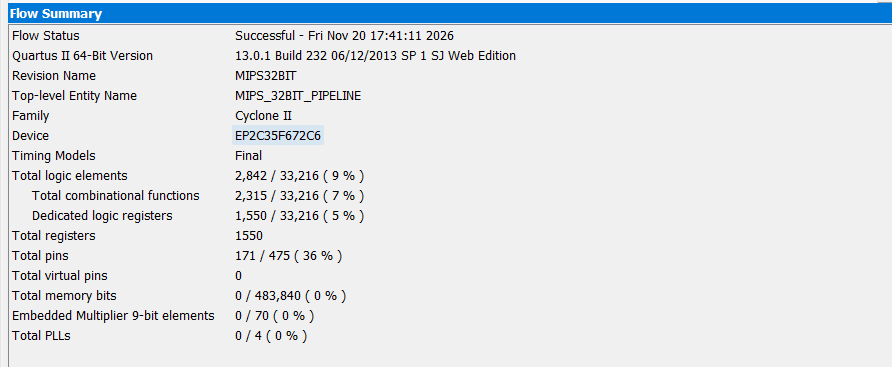
\includegraphics[width=18.5cm]{flow_summary.png}}
    \caption{Kết quả tổng hợp tài nguyên phần cứng (\texttt{Flow Summary}) của bộ vi xử lý \texttt{MIPS\_32BIT\_PIPELINE}}
    \label{fig:quartus_flow_summary}
\end{figure}
\begin{table}[H]
\centering
\caption{Bảng tổng hợp chi phí tài nguyên FPGA và thông số thời gian thực nghiệm trên Cyclone II \texttt{EP2C35F672C6}}
\label{tab:resource_timing_summary}
\setlength{\tabcolsep}{5pt}
\renewcommand{\arraystretch}{1.28}
\resizebox{\textwidth}{!}{%
\begin{tabular}{@{}llcc@{}}
\toprule
\textbf{Nhóm thông số} & \textbf{Chỉ số kỹ thuật (Metric)} & \textbf{Giá trị thực nghiệm} & \textbf{Tỷ lệ / Ghi chú} \\ \midrule
\multirow{5}{*}{\textbf{1. Tài nguyên FPGA}}
 & Tổng số phần tử logic (\texttt{Total logic elements}) & \textbf{2.842 / 33.216} & \textbf{8,56\% ($\approx$ 9\%)} \\
 & \quad -- Hàm logic tổ hợp (\texttt{Total combinational functions}) & \textbf{2.315 / 33.216} & \textbf{6,97\% ($\approx$ 7\%)} (LUT 4-input) \\
 & \quad -- Thanh ghi chuyên dụng (\texttt{Dedicated logic registers}) & \textbf{1.550 / 33.216} & \textbf{4,67\% ($\approx$ 5\%)} (D-Flip-Flops) \\
 & Tổng số Flip-Flops (\texttt{Total registers}) & \textbf{1.550} & Khớp phân tích lý thuyết \\
 & Tổng số chân vào/ra (\texttt{Total pins}) & \textbf{171 / 475} & \textbf{36,00\%} (2 Input + 169 Output) \\ \midrule
\multirow{2}{*}{\textbf{2. Định thời (Timing)}}
 & Tần số xung nhịp tối đa ($f_{\max}$ -- \textit{TimeQuest Slow Model}) & \textbf{62,54 MHz} & Chân xung nhịp \texttt{CLK} \\
 & Chu kỳ xung nhịp tối thiểu ($T_{\min} = 1 / f_{\max}$) & \textbf{15,99 ns} \\ \midrule
\textbf{3. Chu kỳ thực thi}
 & Kiểm thử (\texttt{test\_toan\_dien.asm}) & \begin{tabular}[c]{@{}c@{}}\textbf{27 lệnh tĩnh}\\(23 lệnh thực thi)\end{tabular} & \begin{tabular}[c]{@{}c@{}}Mất \textbf{34 chu kỳ}\\(4 Stall + 3 Flush)\end{tabular} \\ \bottomrule
\end{tabular}%
}
\end{table}

\subsection{Nhận xét và giải trình chi tiết về chi phí tài nguyên FPGA}
\begin{enumerate}
    \item \textbf{Mức độ chiếm dụng tài nguyên thấp và hiệu quả ghép đôi thanh ghi (\textit{Register Packing})}:
    Toàn bộ vi xử lý 32-bit 5 tầng chỉ chiếm \textbf{2.842 / 33.216 LEs ($\approx 9\%$)} dung lượng chip Cyclone II:
    \begin{equation}
        N_{\text{packed\_LE}} = (2.315 + 1.550) - 2.842 = \mathbf{1.023\text{ phần tử logic (LEs)}}
    \end{equation}
    \item \textbf{Giải trình toán học cho con số \texttt{1.550} thanh ghi (\texttt{Dedicated logic registers})}:
    Xét tổng số Flip-Flop đặt trên sơ đồ nguyên lý thiết kế ban đầu:
    \begin{align}
        N_{\text{FF\_thiết\_kế}} &= \underbrace{32}_{\text{PC}} + \underbrace{64}_{\text{IF\_ID\_Reg}} + \underbrace{121}_{\text{ID\_EX\_Reg}} + \underbrace{73}_{\text{EX\_MEM\_Reg}} + \underbrace{71}_{\text{MEM\_WB\_Reg}} \nonumber \\
                                   &\quad + \underbrace{31 \times 32}_{\substack{\text{RegFile (\$1..\$31)}\\\text{(\$0 nối GND = 0 FF)}}} + \underbrace{32 \times 32}_{\text{DMEM (32 words)}} = 361 + 992 + 1.024 = \mathbf{2.377\text{ Flip-Flops}}
    \end{align}
    Sau khi Quartus II tự động rút gọn $24 \times 32 = 768$ Flip-Flops của các thanh ghi \texttt{\$8..\$31} không nối chân \texttt{EN} và gộp $59$ Flip-Flops trùng lặp/hằng số trong các thanh ghi đường ống, số Flip-Flop thực tế còn lại đúng bằng:
    \begin{equation}
        N_{\text{FF\_thực\_tế}} = 2.377 - (768 + 59) = \mathbf{1.550\text{ Flip-Flops}}
    \end{equation}
\end{enumerate}

\section{Phân tích Thời gian (Timing Analysis), Tần số Tối đa \texorpdfstring{$f_{\max}$}{fmax} và Đường dẫn Găng}
Tần số xung nhịp tối đa đạt \textbf{$f_{\max} = 62,54\text{ MHz}$}, tương ứng chu kỳ tối thiểu:
\begin{equation}
    T_{\min} = \frac{1}{f_{\max}} = \frac{1}{62,54 \times 10^6\text{ Hz}} \approx \mathbf{15,99\text{ ns}}
\end{equation}
Nhờ thiết kế \textbf{bộ cộng nhìn trước nhớ phân cấp 2 tầng (\texttt{CLA\_4bit} + \texttt{LCU\_16bit})} trong \texttt{ALU\_32bit.bdf}, độ trễ truyền nhớ 32-bit giảm từ $32$ mức cổng xuống còn $6$ mức cổng logic, giúp tổng độ trễ toàn mạch không vượt quá $T_{\min} = 15,99\text{ ns}$ và đảm bảo mạch hoạt động ổn định tại tần số thiết kế $50\text{ MHz}$ ($T = 20,00\text{ ns}$).
\section{Tính toán Chỉ số CPI, Thời gian Thực thi \texorpdfstring{$T_{\text{exec}}$}{Texec} và So sánh với Kiến trúc Single-Cycle}
Tổng số chu kỳ xung nhịp để hoàn thành chương trình trên Pipeline $k = 5$ tầng là:
\begin{flalign}
    &\text{Total Clock Cycles} = (k - 1) + N_{\text{exec}} + N_{\text{stall}} + N_{\text{flush}} = 4 + 23 + 4 + 3 = \mathbf{34\text{ chu kỳ}} &&
\end{flalign}
\noindent Chỉ số $\text{CPI}$ trung bình và tổng thời gian thực thi thực tế $T_{\text{exec}}$ tại $f_{\max} = 62,54\text{ MHz}$ ($T_{\min} = 15,99\text{ ns}$):
\begin{flalign}
    \text{CPI}_{\text{toàn\_diện}} &= \frac{\text{Total Clock Cycles}}{N_{\text{exec}}} = \frac{34}{23} \approx \mathbf{1,48\text{ chu kỳ/lệnh}} && \\
    T_{\text{exec (tại } f_{\max}\text{)}} &= 34 \times 15,99\text{ ns} = \mathbf{543,66\text{ ns}} && \\
    T_{\text{exec (tại } 50\text{ MHz)}} &= 34 \times 20,00\text{ ns} = \mathbf{680,00\text{ ns}} &&
\end{flalign}
\vspace{-0.25cm}
\begin{table}[H]
\centering
\caption{Đối chiếu hiệu suất Single-Cycle và Pipeline 5 tầng ($N_{\text{exec}} = 23$ lệnh)}
\label{tab:performance_comparison}
\setlength{\tabcolsep}{6pt}
\renewcommand{\arraystretch}{1.05}
\resizebox{0.96\textwidth}{!}{%
\begin{tabular}{@{}lcc@{}}
\toprule
\textbf{Chỉ số đánh giá hiệu năng} & \textbf{1. MIPS Single-Cycle (Tham chiếu)} & \textbf{2. Pipeline 5 tầng (Thiết kế Đồ án)} \\ \midrule
Tần số xung nhịp tối đa ($f_{\max}$) & $\sim 16,00\text{ MHz}$ & \textbf{62,54 MHz} \\
Chu kỳ xung nhịp tối thiểu ($T_{\min}$) & $62,50\text{ ns}$ & \textbf{15,99 ns} \\
Số chu kỳ trễ do Hazard ($N_{\text{stall}} + N_{\text{flush}}$) & $0\text{ chu kỳ}$ & \textbf{7 chu kỳ (4 Stall + 3 Flush)} \\
Tổng số chu kỳ hoàn thành ($\text{Total Cycles}$) & $23\text{ chu kỳ}$ & \textbf{4 + 23 + 7 = 34 chu kỳ} \\
Chỉ số $\text{CPI}$ trung bình thực tế & $1,00\text{ chu kỳ/lệnh}$ & \textbf{34 / 23 = 1,48 chu kỳ/lệnh} \\
Tổng thời gian thực thi ($T_{\text{exec}}$ tại $f_{\max}$) & $23 \times 62,50 = \mathbf{1.437,50\text{ ns}}$ & $34 \times 15,99 = \mathbf{543,66\text{ ns}}$ \\
\textbf{Hệ số tăng tốc tổng thể (\textit{Speedup})} & \textbf{1,00$\times$ (Cơ sở)} & \textbf{2,64$\times$ (Nhanh gấp 2,64 lần!)} \\ \bottomrule
\end{tabular}%
}
\end{table}
% ==============================================================================
% CHƯƠNG 5: KẾT LUẬN VÀ HƯỚNG PHÁT TRIỂN
% ==============================================================================
\chapter{Kết Luận và Hướng Phát Triển}

\section{Kết luận tổng hợp các ưu điểm của thiết kế}
\begin{enumerate}
    \item \textbf{Hoàn thiện đầy đủ Datapath và Control Unit cho 15 lệnh cốt lõi}: Thực thi chính xác 3 định dạng lệnh R-type (\texttt{add, sub, and, or, nor, slt, sll, srl, nop}), I-type (\texttt{addi, ori, lw, sw, beq, bne}) và J-type (\texttt{j}), bảo vệ cứng thanh ghi \texttt{\$0 = 0}.
    \item \textbf{Tối ưu tốc độ tính toán nhờ Bộ cộng Nhìn trước nhớ Phân cấp (\textit{Carry Lookahead Adder -- CLA})}: Kiến trúc CLA 2 cấp (\texttt{CLA\_4bit} + \texttt{LCU\_16bit}) rút ngắn đường găng tầng \texttt{EX}, nâng tần số hoạt động tối đa lên \textbf{$f_{\max} = 62,54\text{ MHz}$} ($T_{\min} = 15,99\text{ ns}$).
    \item \textbf{Triệt tiêu tối đa chu kỳ Stall nhờ \texttt{Forwarding\_Unit} và kỹ thuật ghi sườn xuống \texttt{CLK\_N}}: Giải quyết trọn vẹn xung đột RAW đơn, xung đột kép (\textit{Double Data Hazard}) và tự động hóa chu trình ghi nửa đầu -- đọc nửa sau chu kỳ tại \texttt{RegFile}.
    \item \textbf{Giảm Branch Penalty xuống 1 chu kỳ nhờ \texttt{Branch\_Unit} tại tầng \texttt{ID}}: Đạt $\text{CPI} = 1,48$ và tăng tốc độ thực thi tổng thể gấp \textbf{2,64 lần} so với kiến trúc MIPS đơn chu kỳ, trong khi chỉ tiêu tốn \textbf{9\% Logic Elements} (\texttt{2.842 / 33.216} LEs) và \textbf{5\% Registers} (\texttt{1.550} Flip-Flops).
\end{enumerate}
\section{Hướng phát triển của đề tài}
\begin{itemize}
    \item Chuyển đổi \texttt{IMEM} và \texttt{DMEM} sang sử dụng khối RAM nội chuyên dụng \textbf{\texttt{M4K}} trên chip Cyclone II và bổ sung bộ nhớ đệm \textbf{I-Cache / D-Cache}.
    \item Bổ sung khối nhân/chia phần cứng (\texttt{mult, div}) và giao tiếp ngoại vi Memory-Mapped I/O (LED 7 đoạn) trên bo mạch thực tế \textbf{Altera DE2}.
\end{itemize}

% ==============================================================================
% TÀI LIỆU THAM KHẢO
% ==============================================================================
\begin{thebibliography}{9}
\bibitem{patterson}
David A. Patterson, John L. Hennessy, \textit{Computer Organization and Design: The Hardware/Software Interface}, 5th Edition, Morgan Kaufmann, 2013.

\bibitem{harris}
David Money Harris, Sarah L. Harris, \textit{Digital Design and Computer Architecture}, 2nd Edition, Morgan Kaufmann, 2012.

\bibitem{quartus}
Altera Corporation, \textit{Quartus II Handbook Version 13.0 SP1}, 2013.
\end{thebibliography}

\end{document}
